\documentclass[handout]{beamer}
\usepackage{graphicx}
\usepackage{xcolor}
\usepackage{multirow}
\setbeamertemplate{blocks}[rounded][shadow=true] % estilo de bloque
\setbeamercolor{block body}{bg=gray!20, fg=black}  % fondo y texto
\setbeamercolor{block title}{bg=blue!20, fg=black} % título
%Information to be included in the title page:
\title{Procesos Markovianos de Decisión}
\author{Daniela Pucci de Farias}
\institute{Universidad Torcuato Di Tella}
\date{June 2025}

\begin{document}

\frame{\titlepage}

\begin{frame}{Trabajo Práctico}
\begin{itemize}
\item Finalizar formación de grupos
\item 30 de junio: Entregar propuesta de proyecto y modelo inicial de MDP (máximo 2 páginas)
\end{itemize}
\end{frame}

\begin{frame}{Clase 3}
\begin{itemize}
\item MDPs con horizonte infinito
\begin{itemize}
\item Ecuación de Bellman
\item Iteración de valor
\item Iteración de políticas
\item Función de utilidad
\end{itemize}
\item Aplicaciones
\begin{itemize}
\item Política de pesca
\item Optimización de portafolio
\end{itemize}
\end{itemize}
\end{frame}

\begin{frame}{MDPs, Función Valor, Políticas}
\begin{itemize}
\item {\bf Proceso markoviano de decisión (MDP)}:
\begin{itemize}
\item tupla $(S,P,r,A)$
\item<2-> matriz de transición y recompensa dependen de la acción $a \in A$: $P_a$, $r_a$
\end{itemize}
\item<3-> $u_t: S \mapsto A$ es una {\bf política} indicando, para cada periodo $t$ y estado $x$, una acción $a = u_t(x)$.
\item<4-> {\bf Función valor} $V^*$ indica la recompensa esperada empezando em cada estado:
$$
V_t^*(x) = \max_u \left[\sum_{\tau=t}^T \alpha^{\tau-t} r_u(x)|x_t = x\right]
$$
\begin{itemize}
\item $\alpha \in [0,1]$ es el factor de descuento 
\end{itemize}
\end{itemize}    
\end{frame}


\begin{frame}{Programación Dinámica Para MDPs}
\begin{itemize}
\item Calculamos la funcion valor $V^*$ recursivamente:
\begin{center}
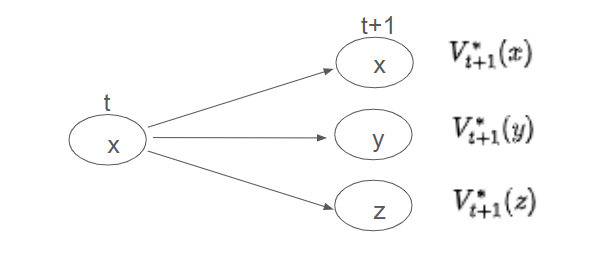
\includegraphics[width=0.6\textwidth]{../Images/OtherFigures/Bellman.png}
\end{center}
\visible<2->{
\begin{block}{Programación Dinámica con Horizonte T}
\begin{enumerate}
\item<3-> Hacemos $t = T$. Calculamos $V_T^*(x) = \max_a r_a(x).$
\item<4-> Hacemos $t = t-1$. Calculamos 
$V^*_t(x) =  \max\limits_{a \in A} \left\{r_a(x)+\alpha \sum_y P_a(x,y) V_{t+1}^*(y)\right\}$.
\item<5-> Si $t = 0$, fin. Si no, volvemos al paso 2.
\end{enumerate}
\end{block}}
\item<6-> Derivamos la política óptima a partir de la función valor $V^*$:
$$
u^*_t(x) = \arg\max\limits_{a \in A} \left\{r_a(x)+\alpha \sum_y P_a(x,y) V_{t+1}^*(y)\right\} 
$$
\end{itemize}
\end{frame}

\begin{frame}{Ejemplo: Pesca de Salmones}
Cada año, necesitamos decidir cuánto salmón pescar en una determinada área. Cada salmón genera una ganancia fija. Pero si pescamos demasiados salmones en un año, eso impactará en la cantidad de salmones disponibles en el año siguiente. Debemos decidir cuánto pescar a cada año para maximizar la ganancia. 

\vspace{0.5cm}
Cómo modelamos ese problema?

\vspace{0.5cm}
\visible<2->{Vamos a considerar una versión simplificada para visualizar el proceso:
\begin{itemize}
\item<3-> a cada año, decidimos solo si pescar o no una cierta proporción de salmones;
\item<4-> consideramos 4 estados para a población de salmones: vacío, bajo, mediano, alto.
\end{itemize}}
\end{frame}

\begin{frame}{Pesca de Salmones: Modelo}
\begin{center}
\mode<beamer>{
\only<1>{
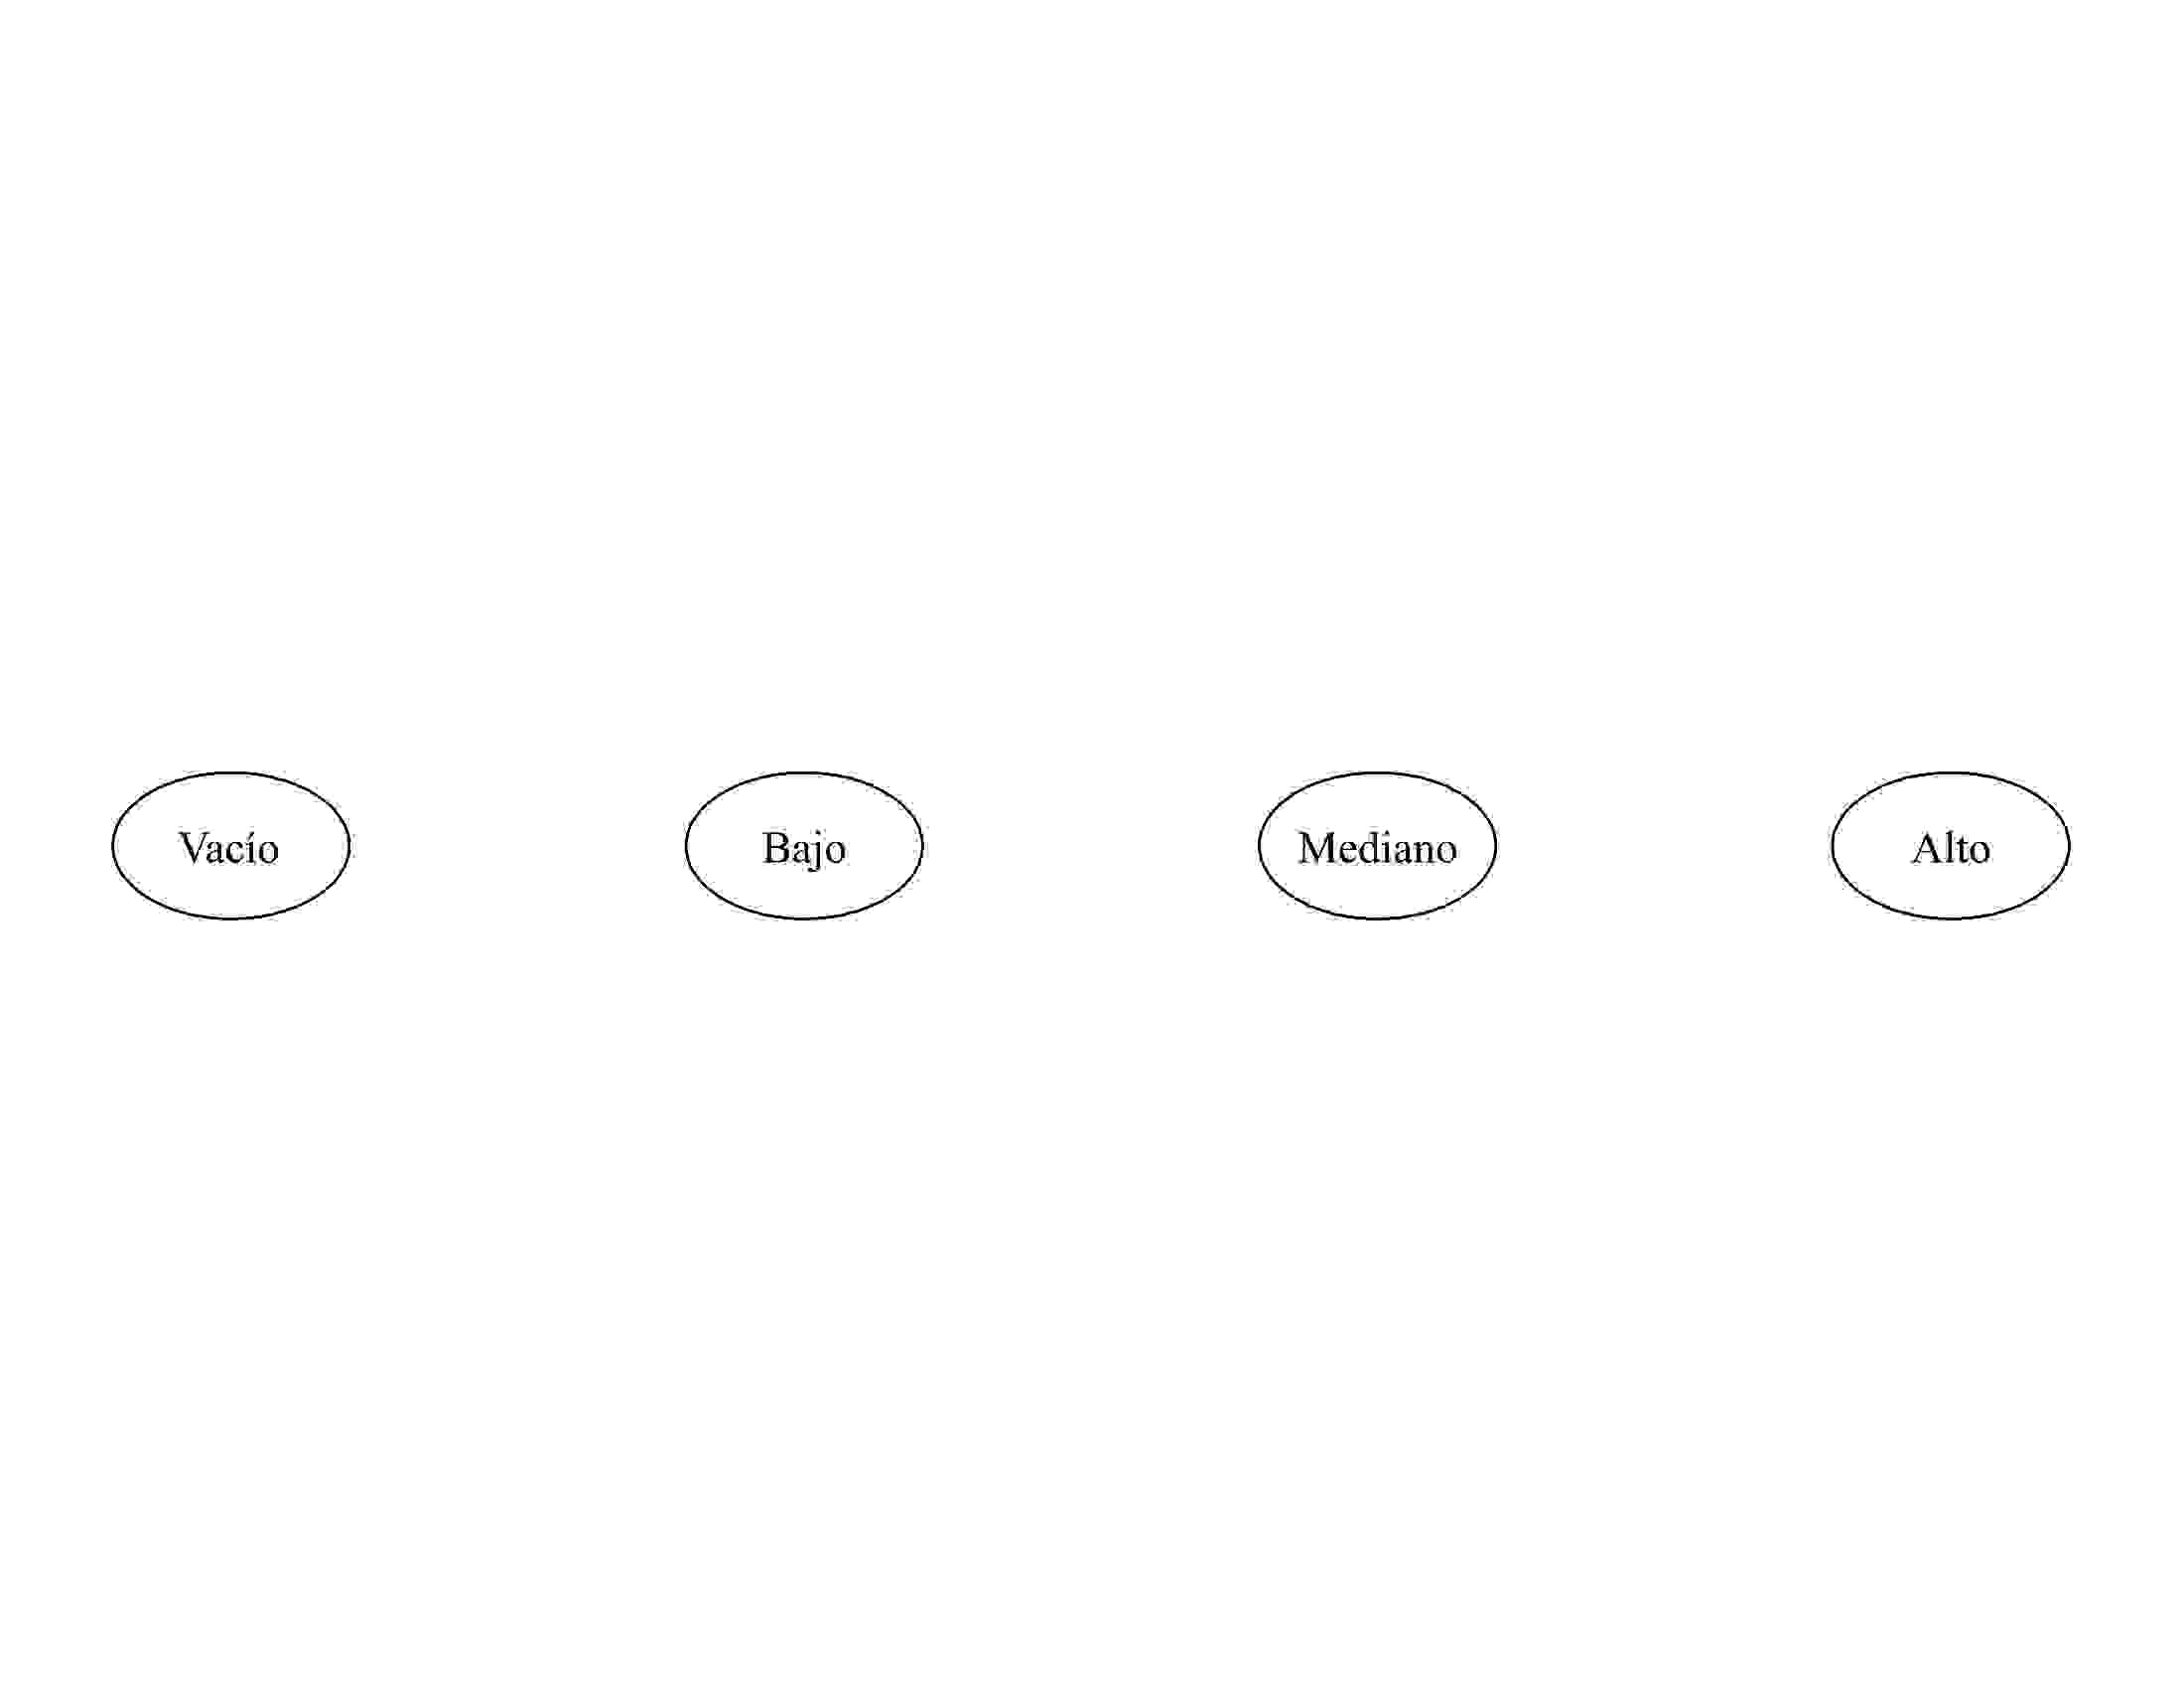
\includegraphics[width=1\textwidth]{../Images/SalmonFishing/SalmonFishing1.jpg}}
\only<2>{
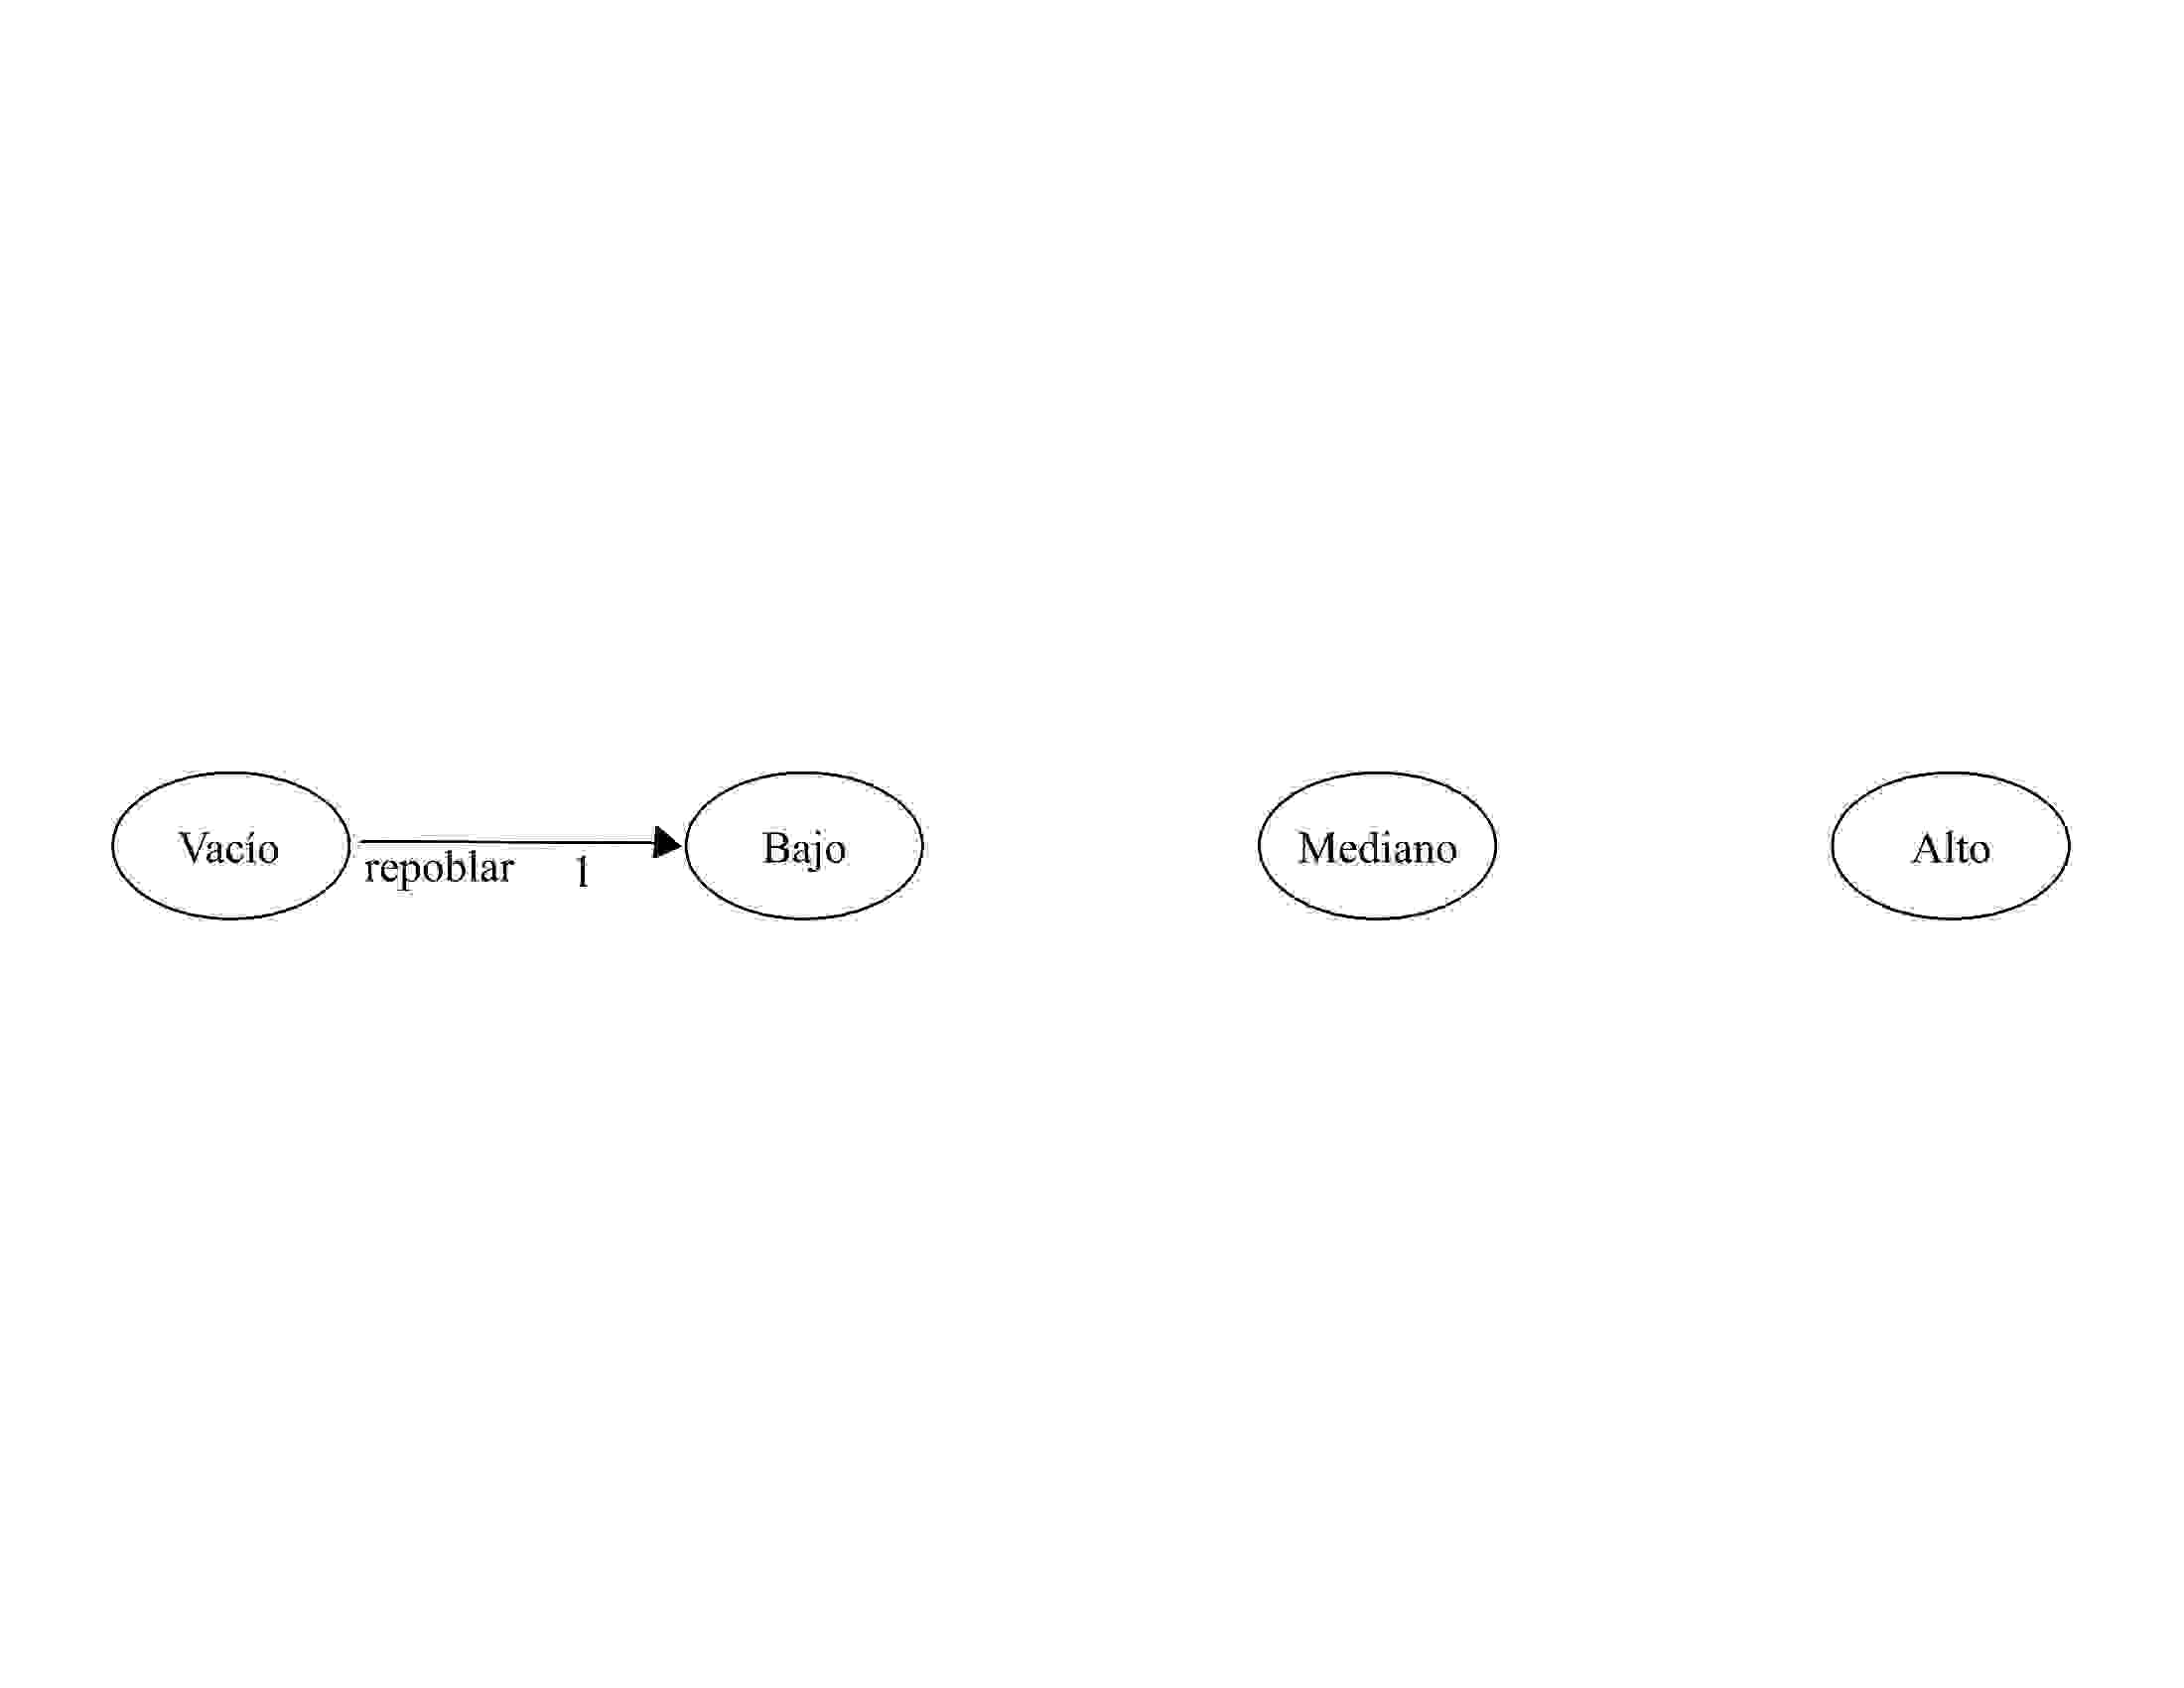
\includegraphics[width=1\textwidth]{../Images/SalmonFishing/SalmonFishing2.jpg}}
\only<3>{
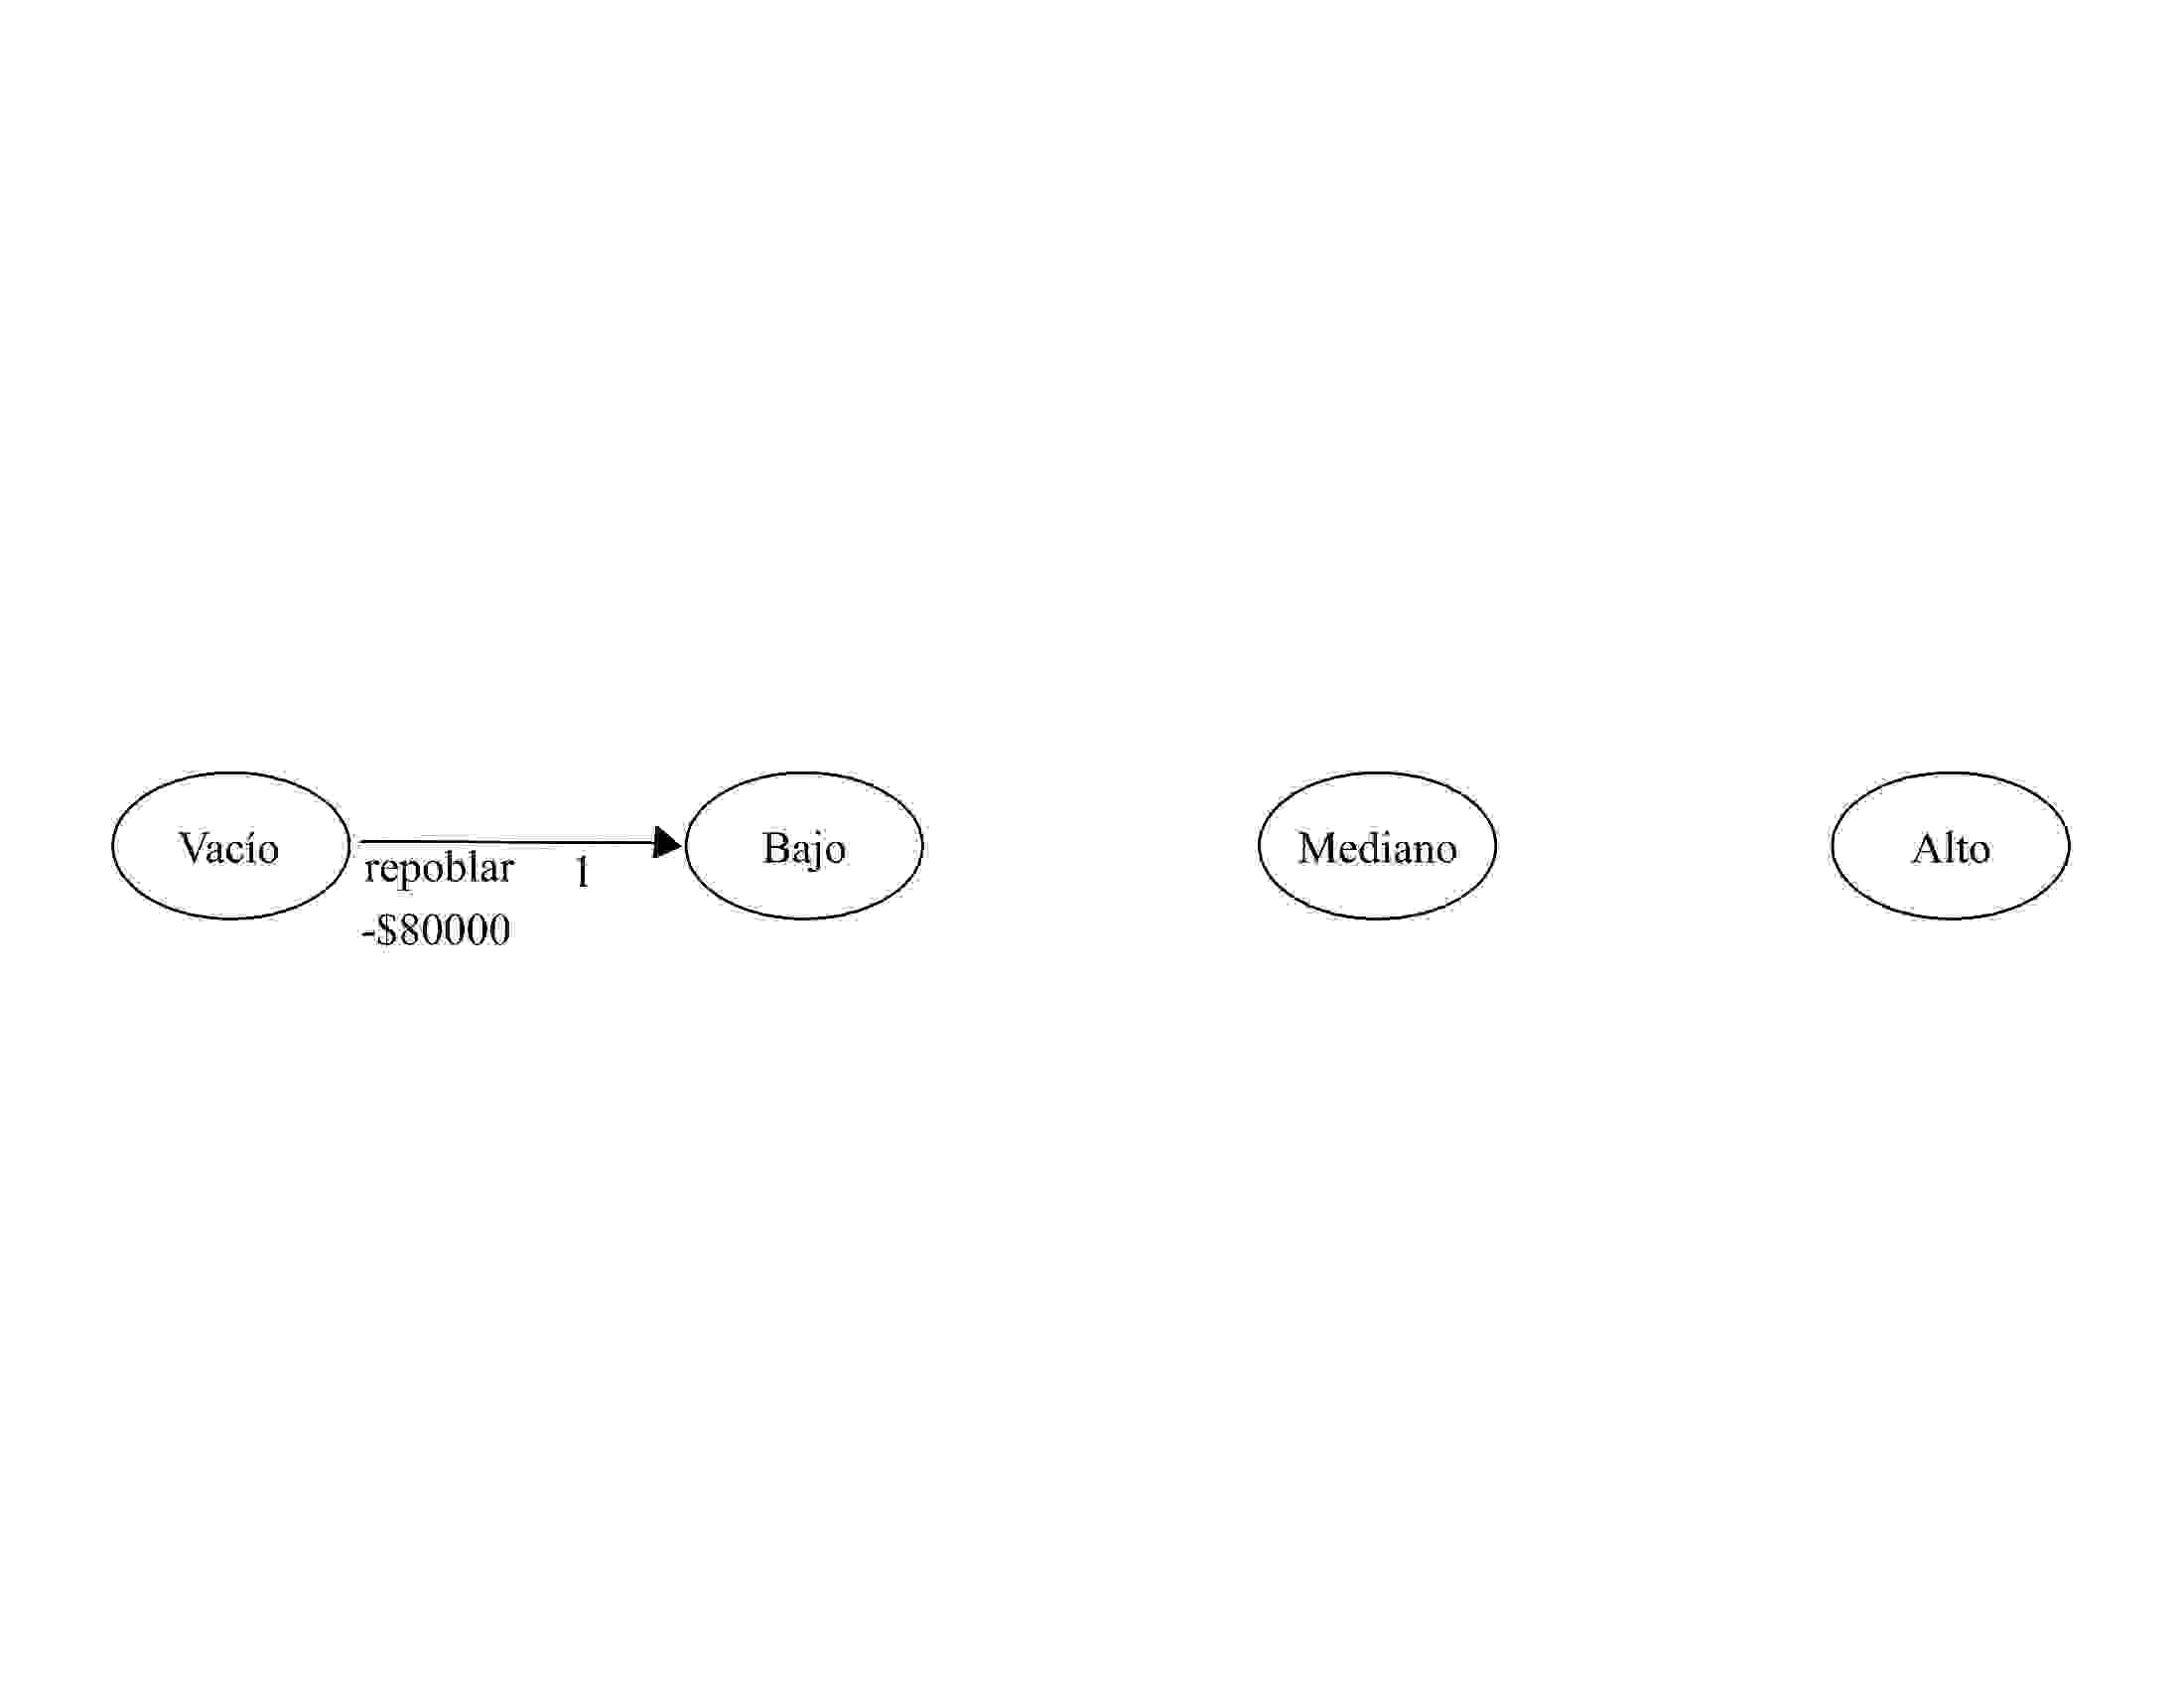
\includegraphics[width=1\textwidth]{../Images/SalmonFishing/SalmonFishing3.jpg}}
\only<4>{
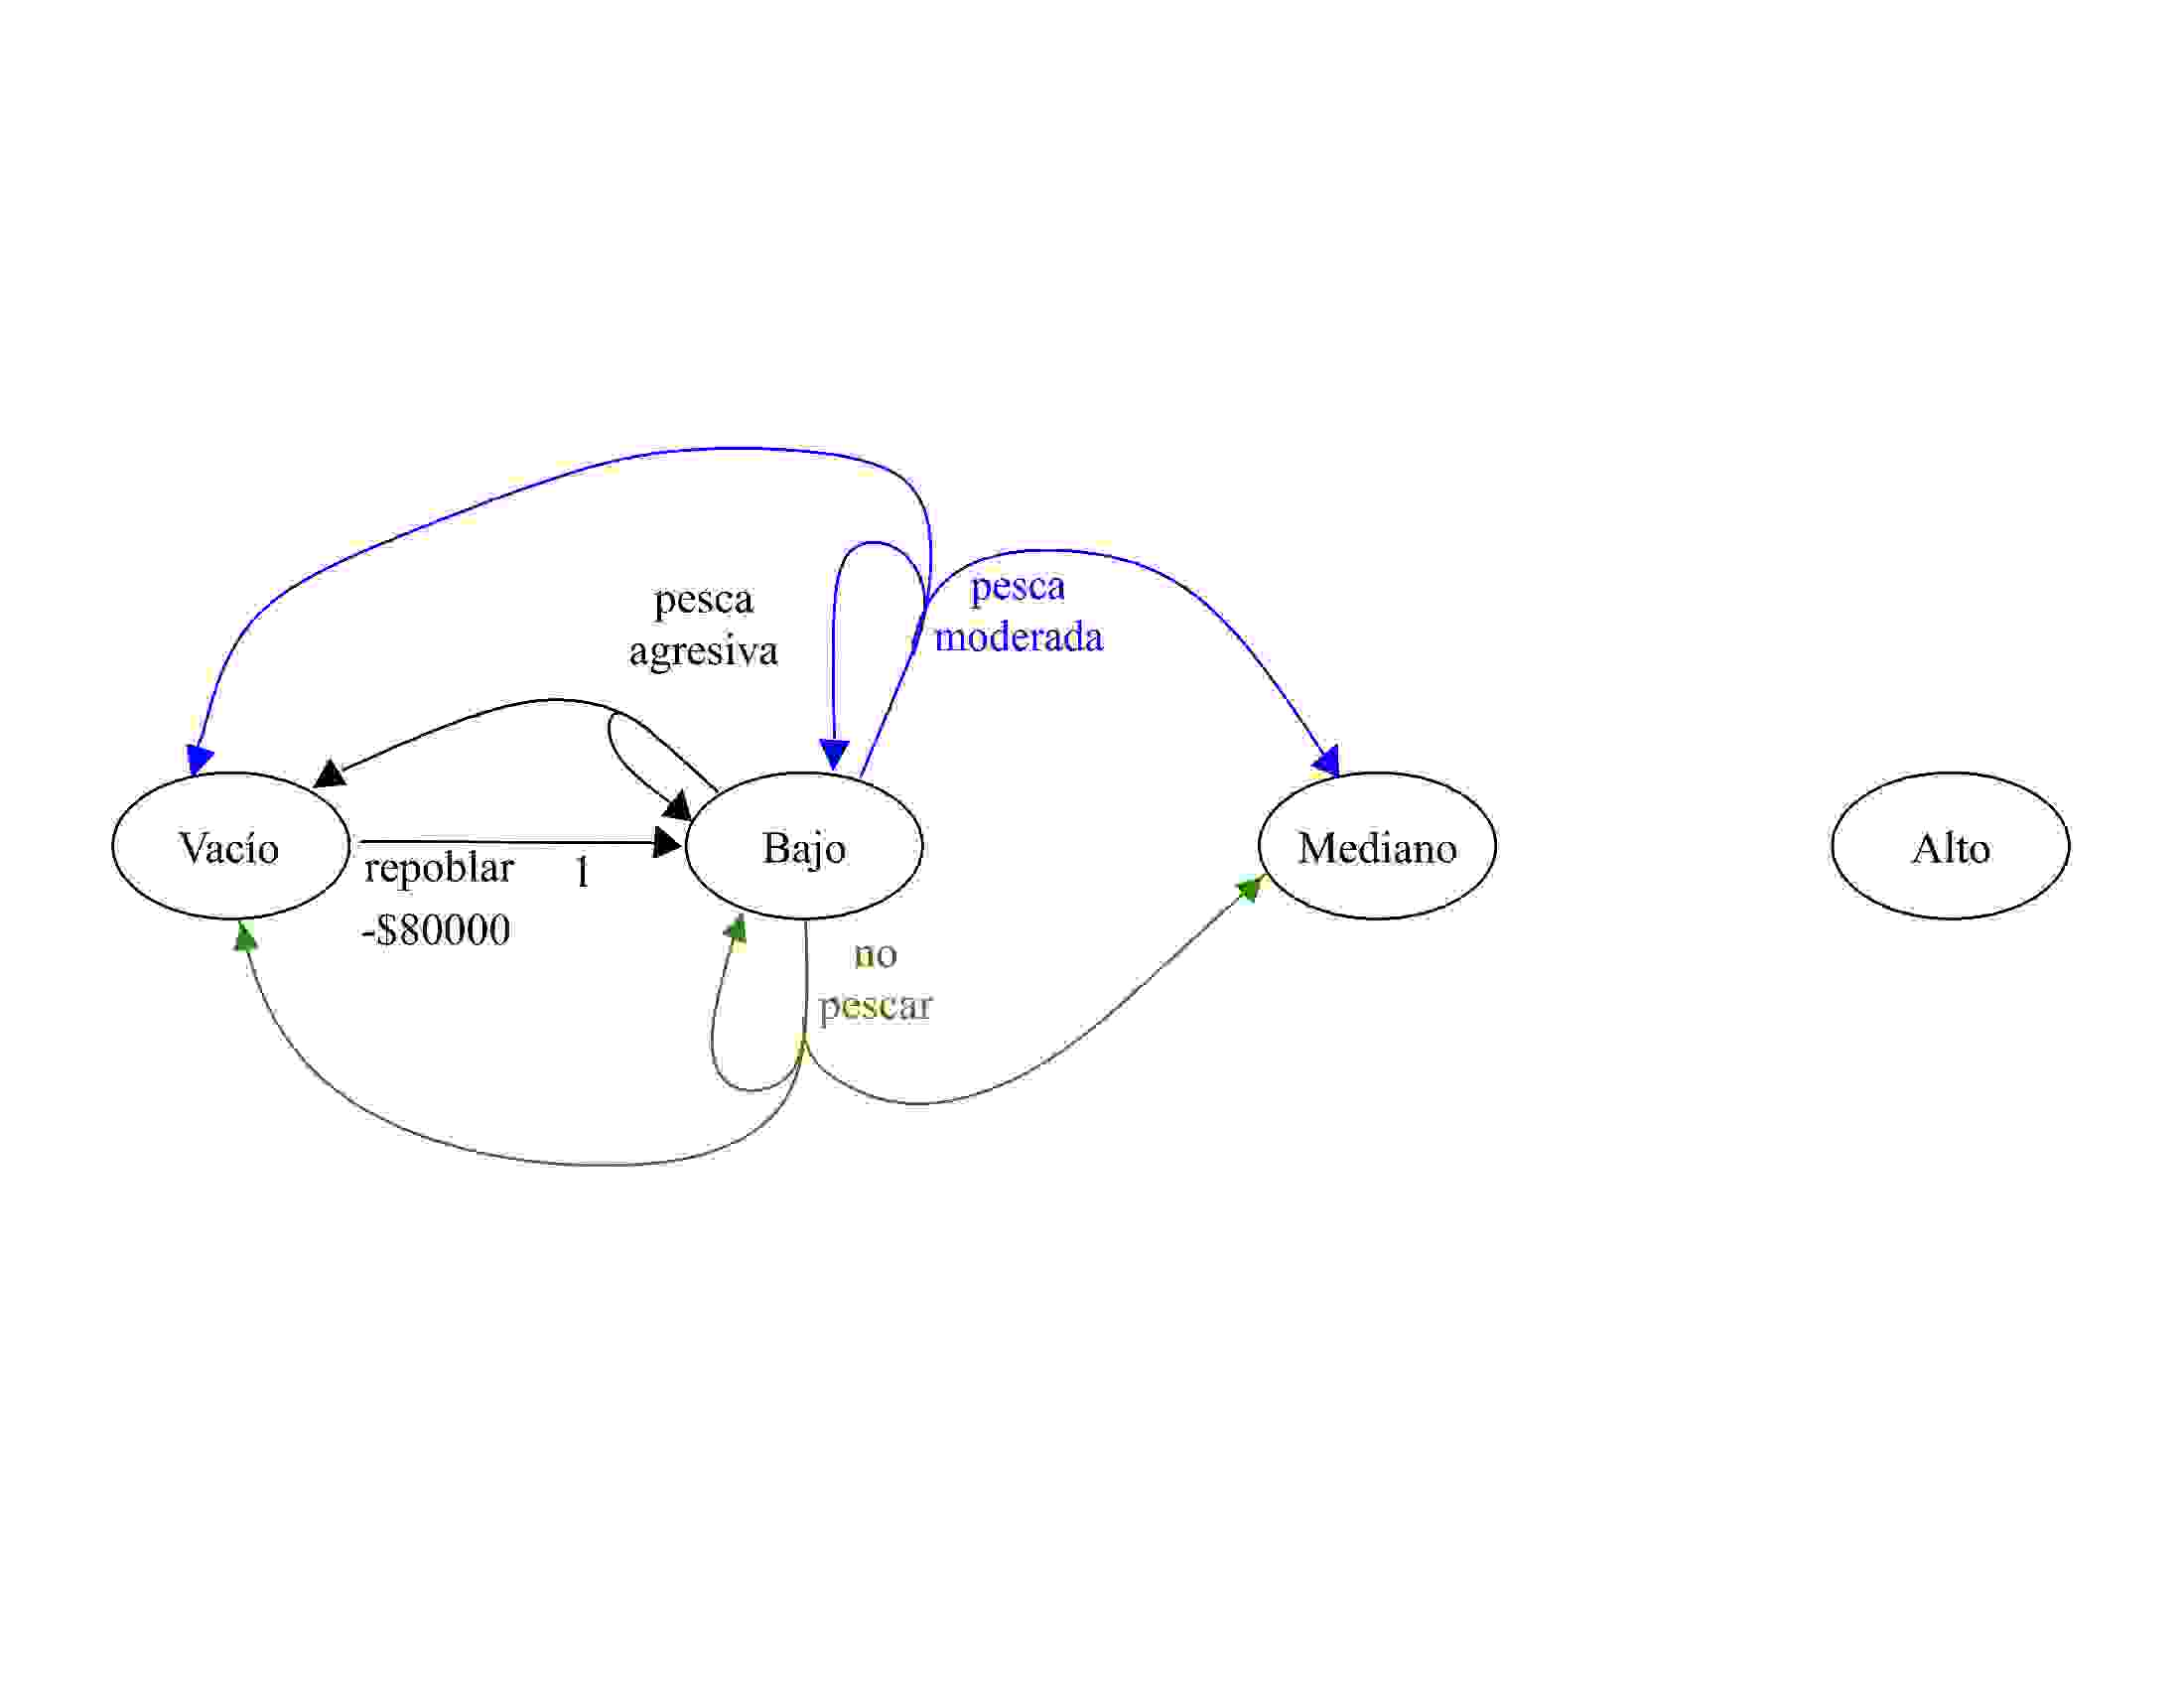
\includegraphics[width=1\textwidth]{../Images/SalmonFishing/SalmonFishing4.jpg}}
\only<5>{
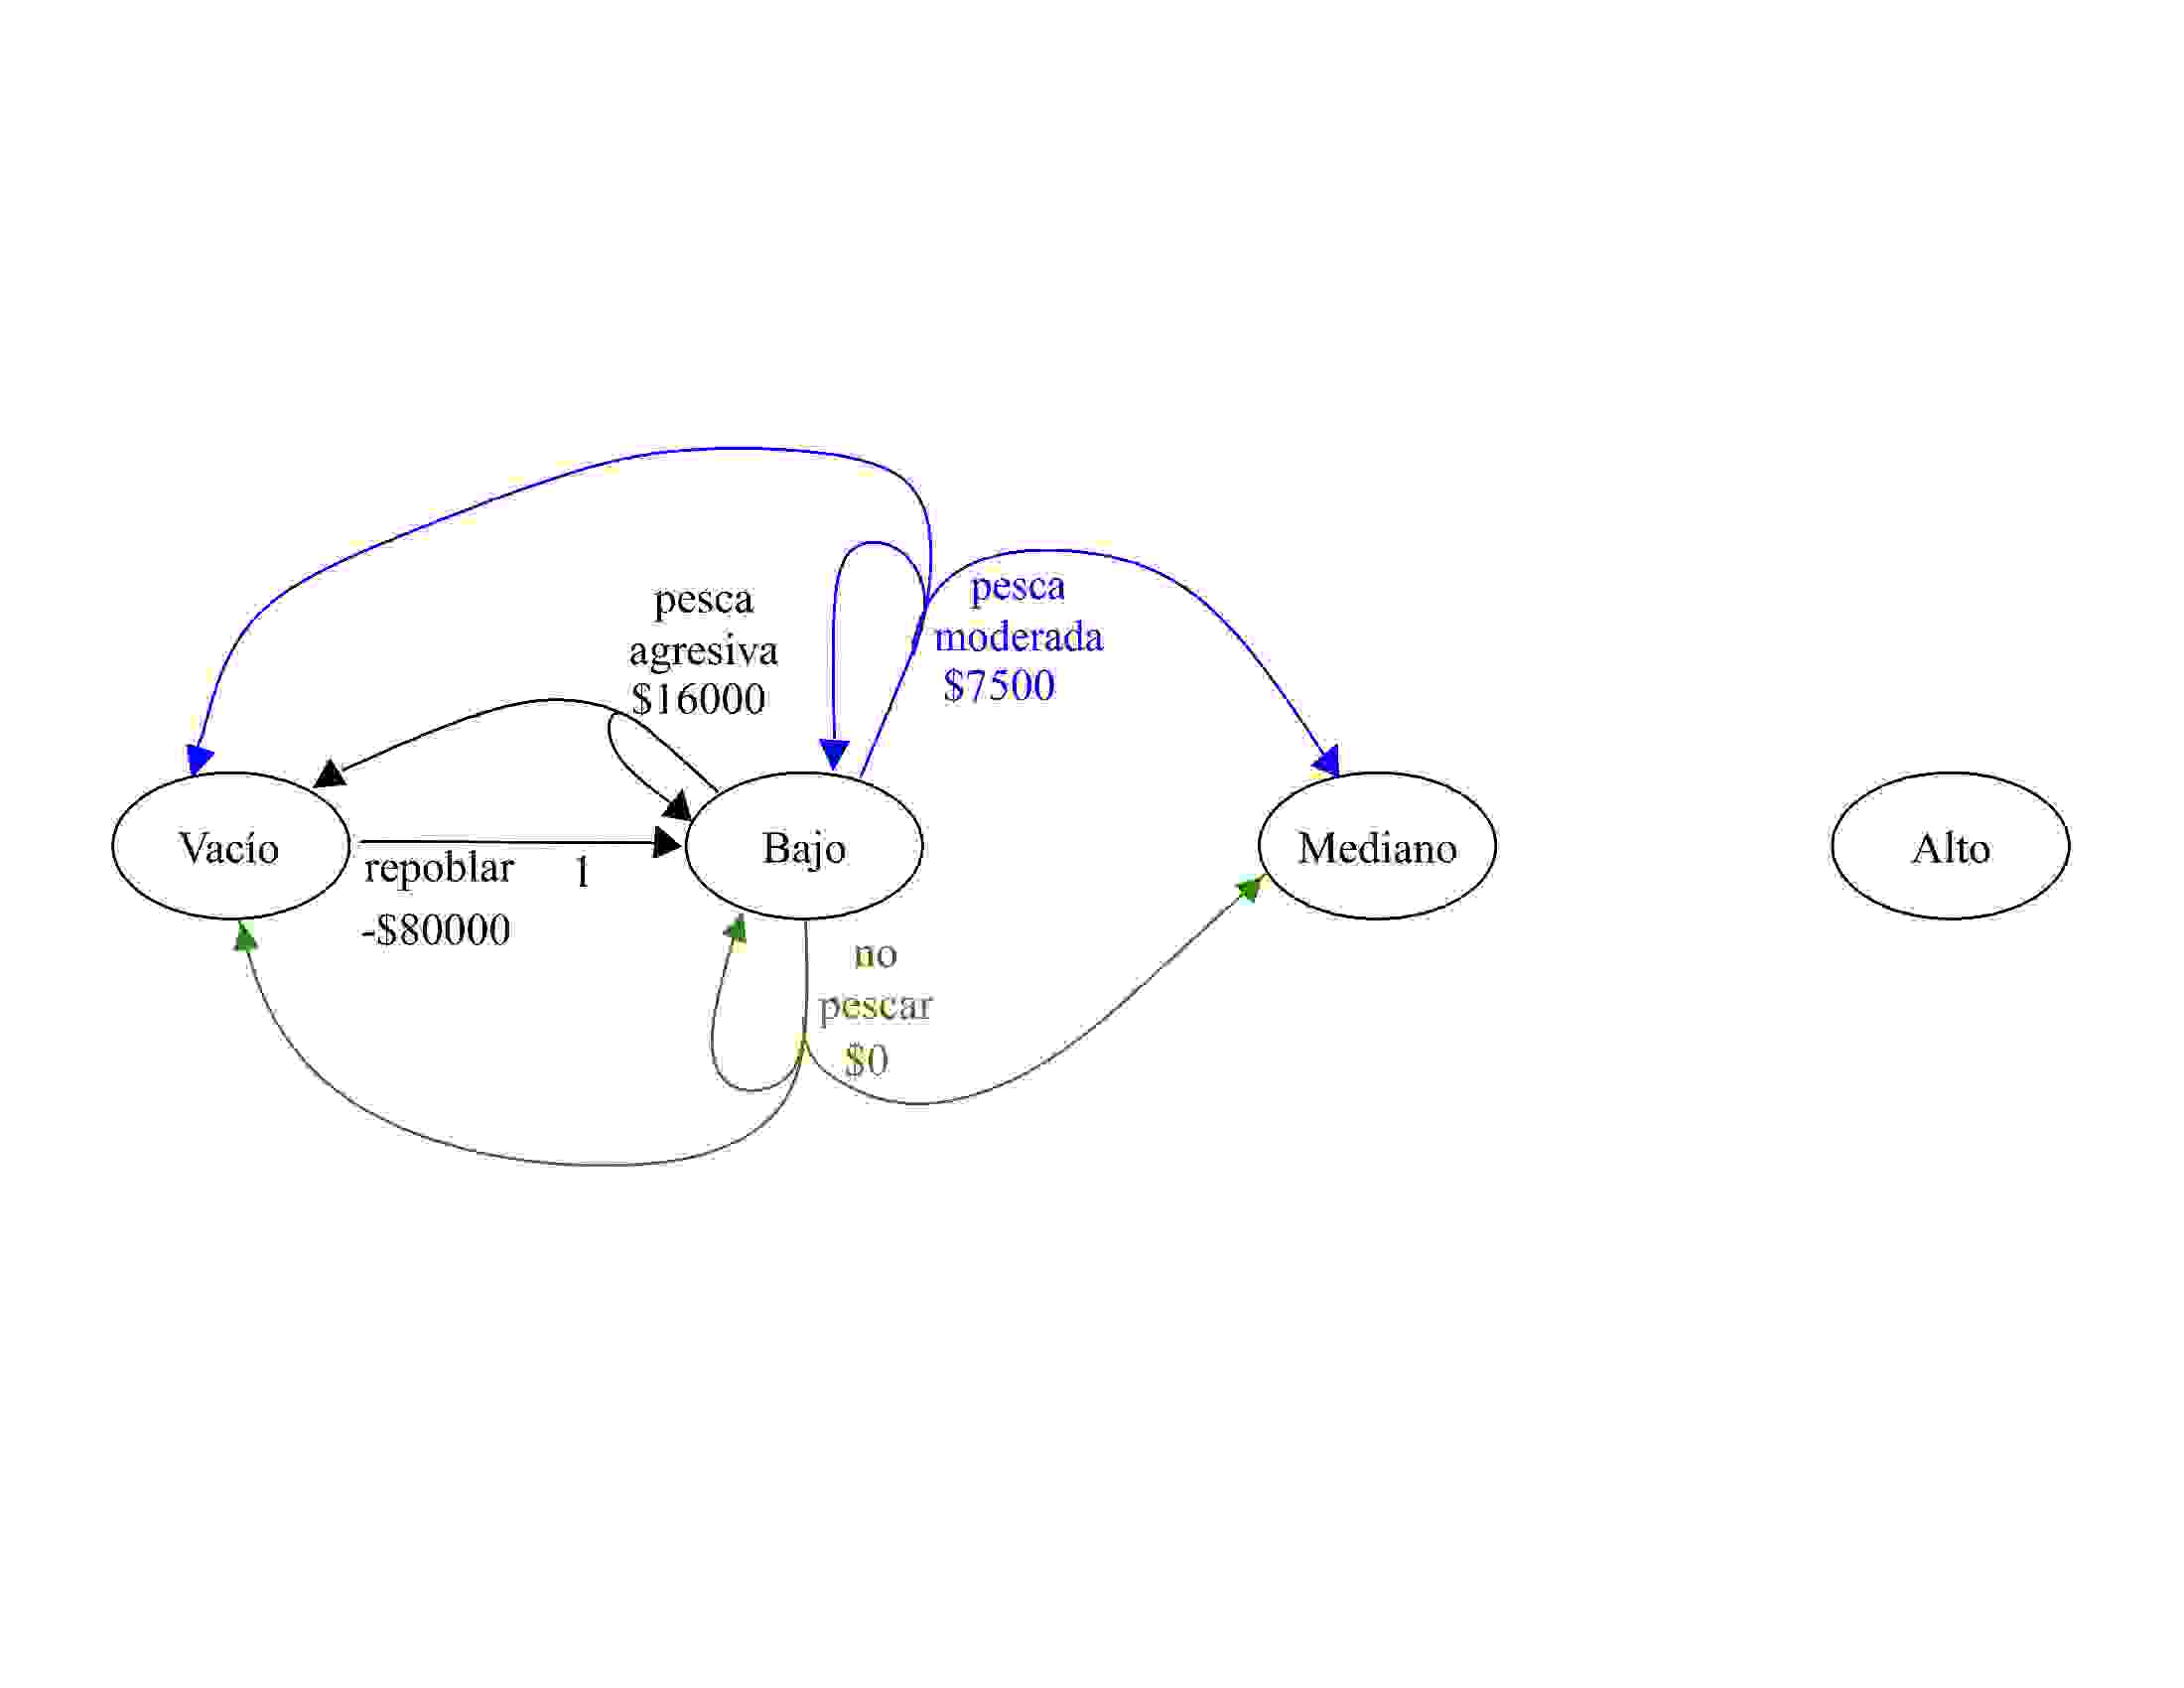
\includegraphics[width=1\textwidth]{../Images/SalmonFishing/SalmonFishing5.jpg}}
\only<6>{
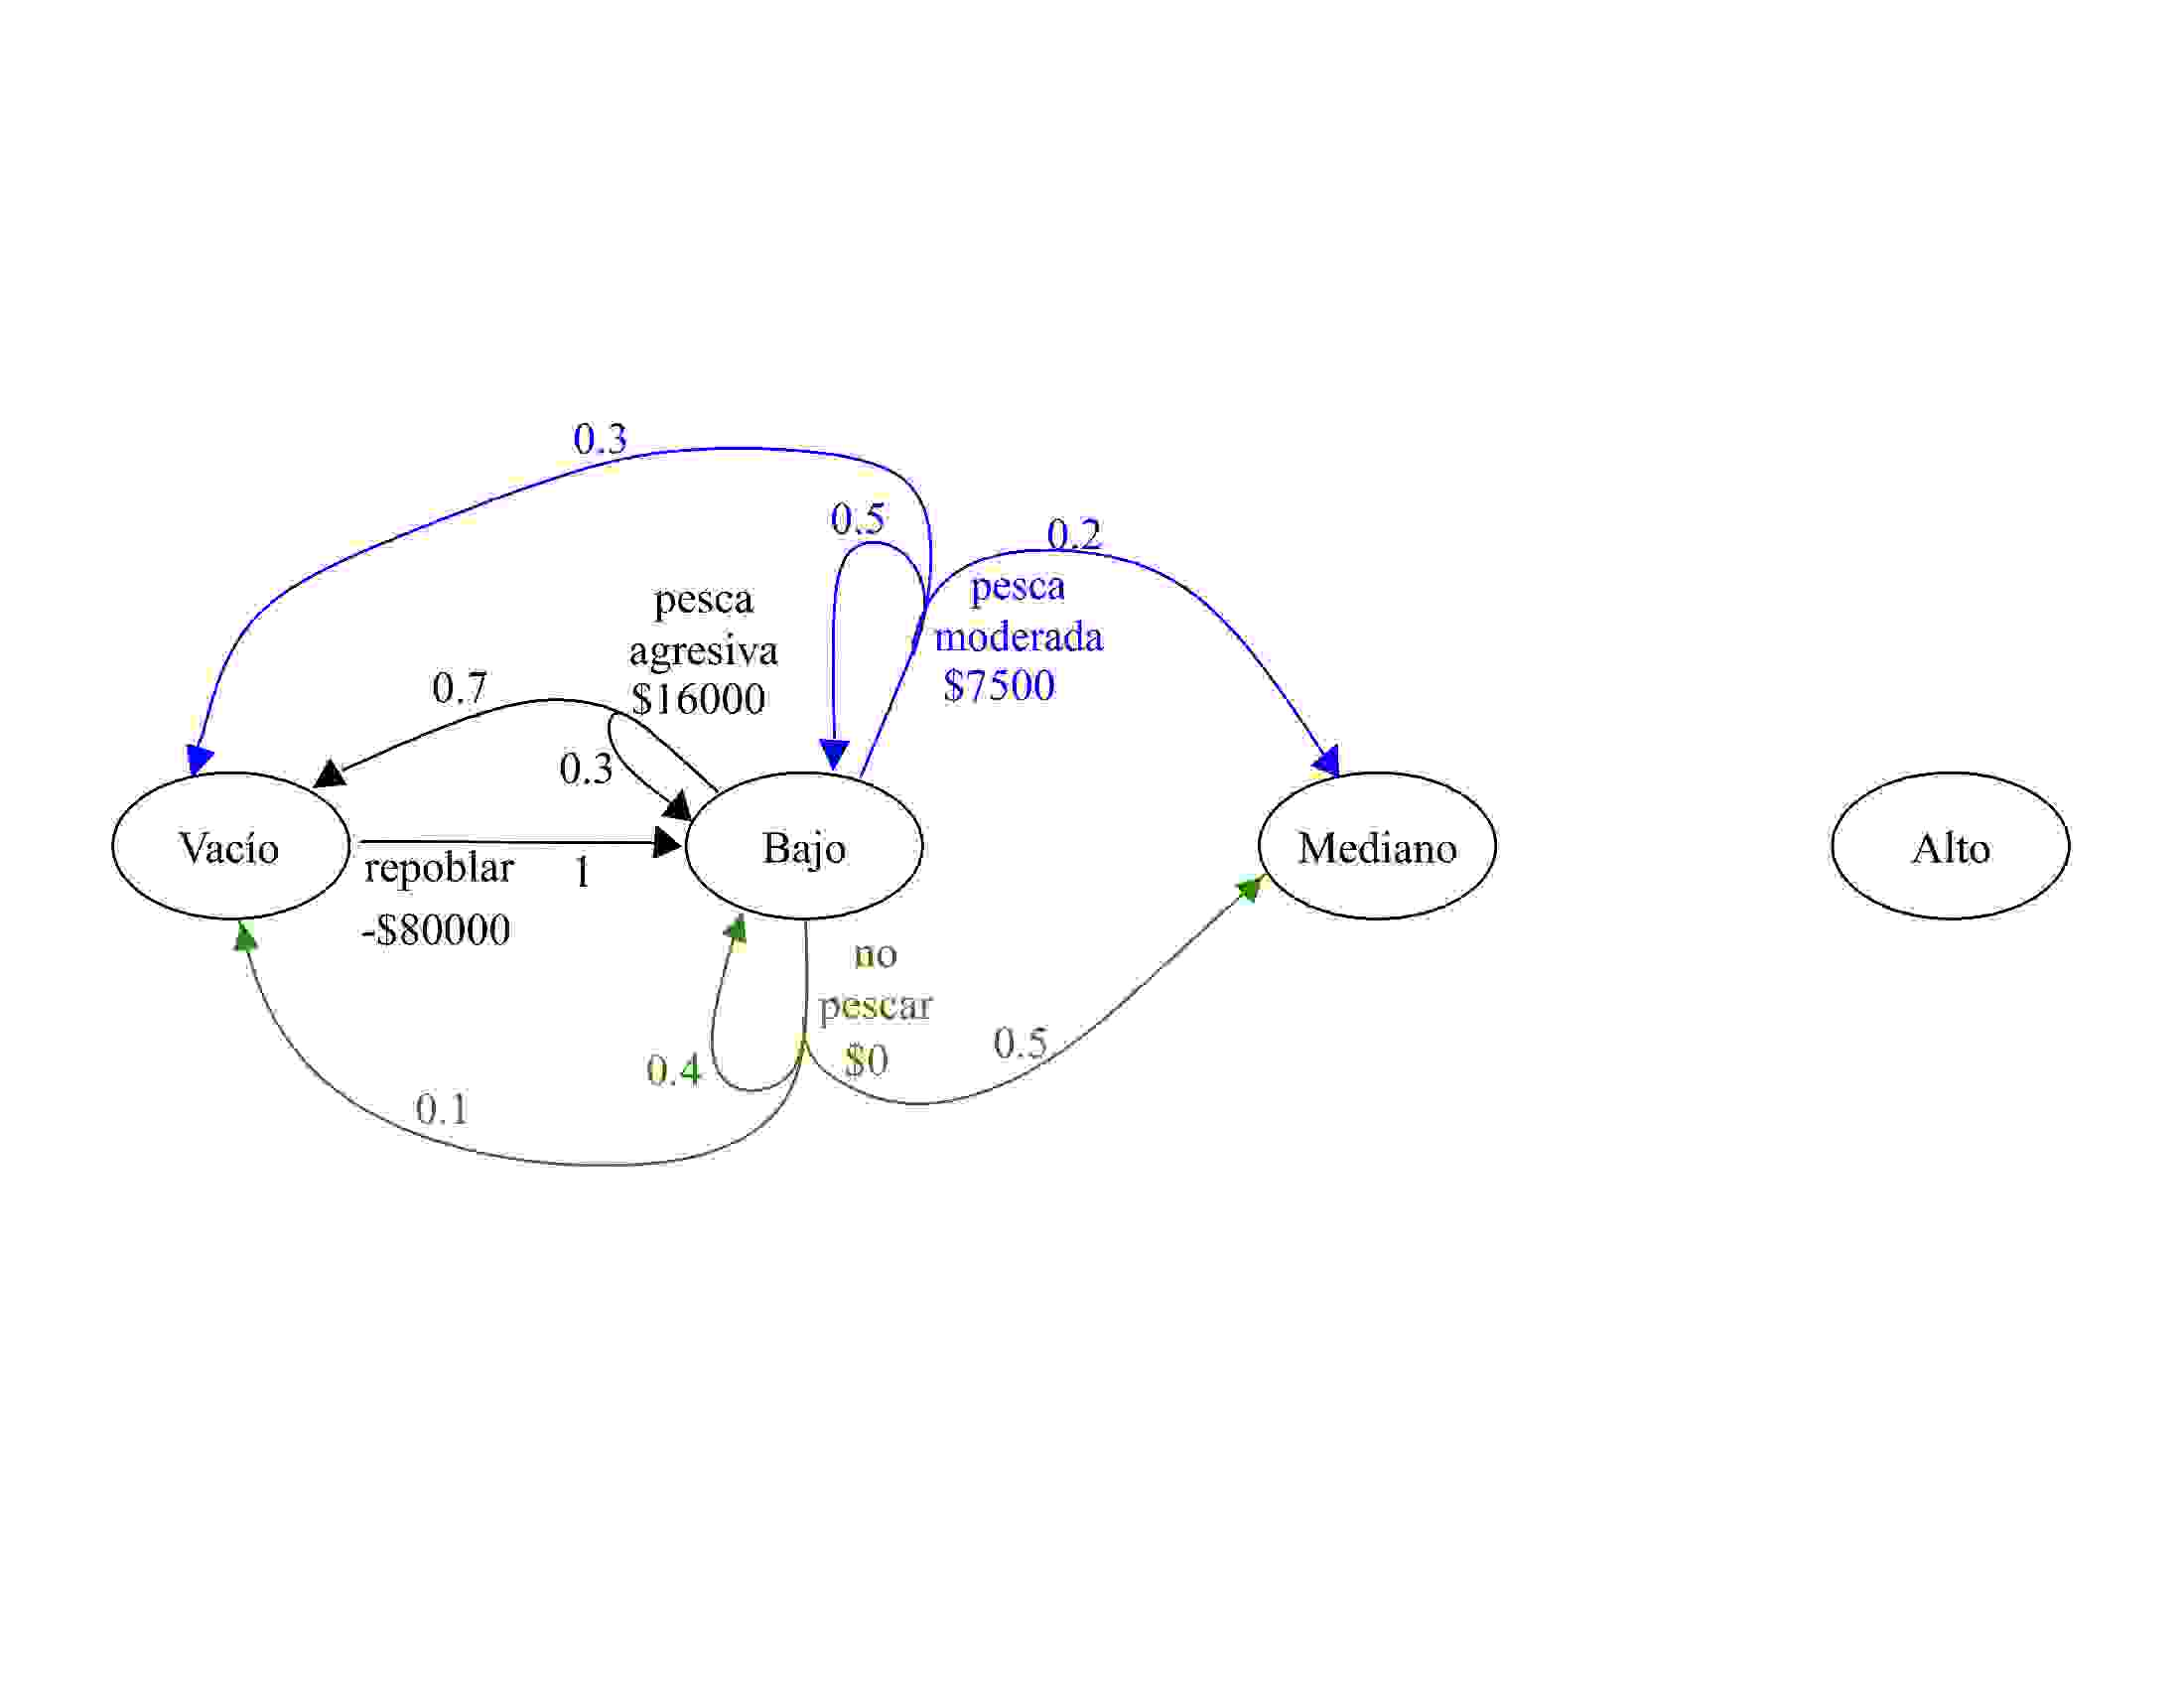
\includegraphics[width=1\textwidth]{../Images/SalmonFishing/SalmonFishing6.jpg}}}
\only<7->{
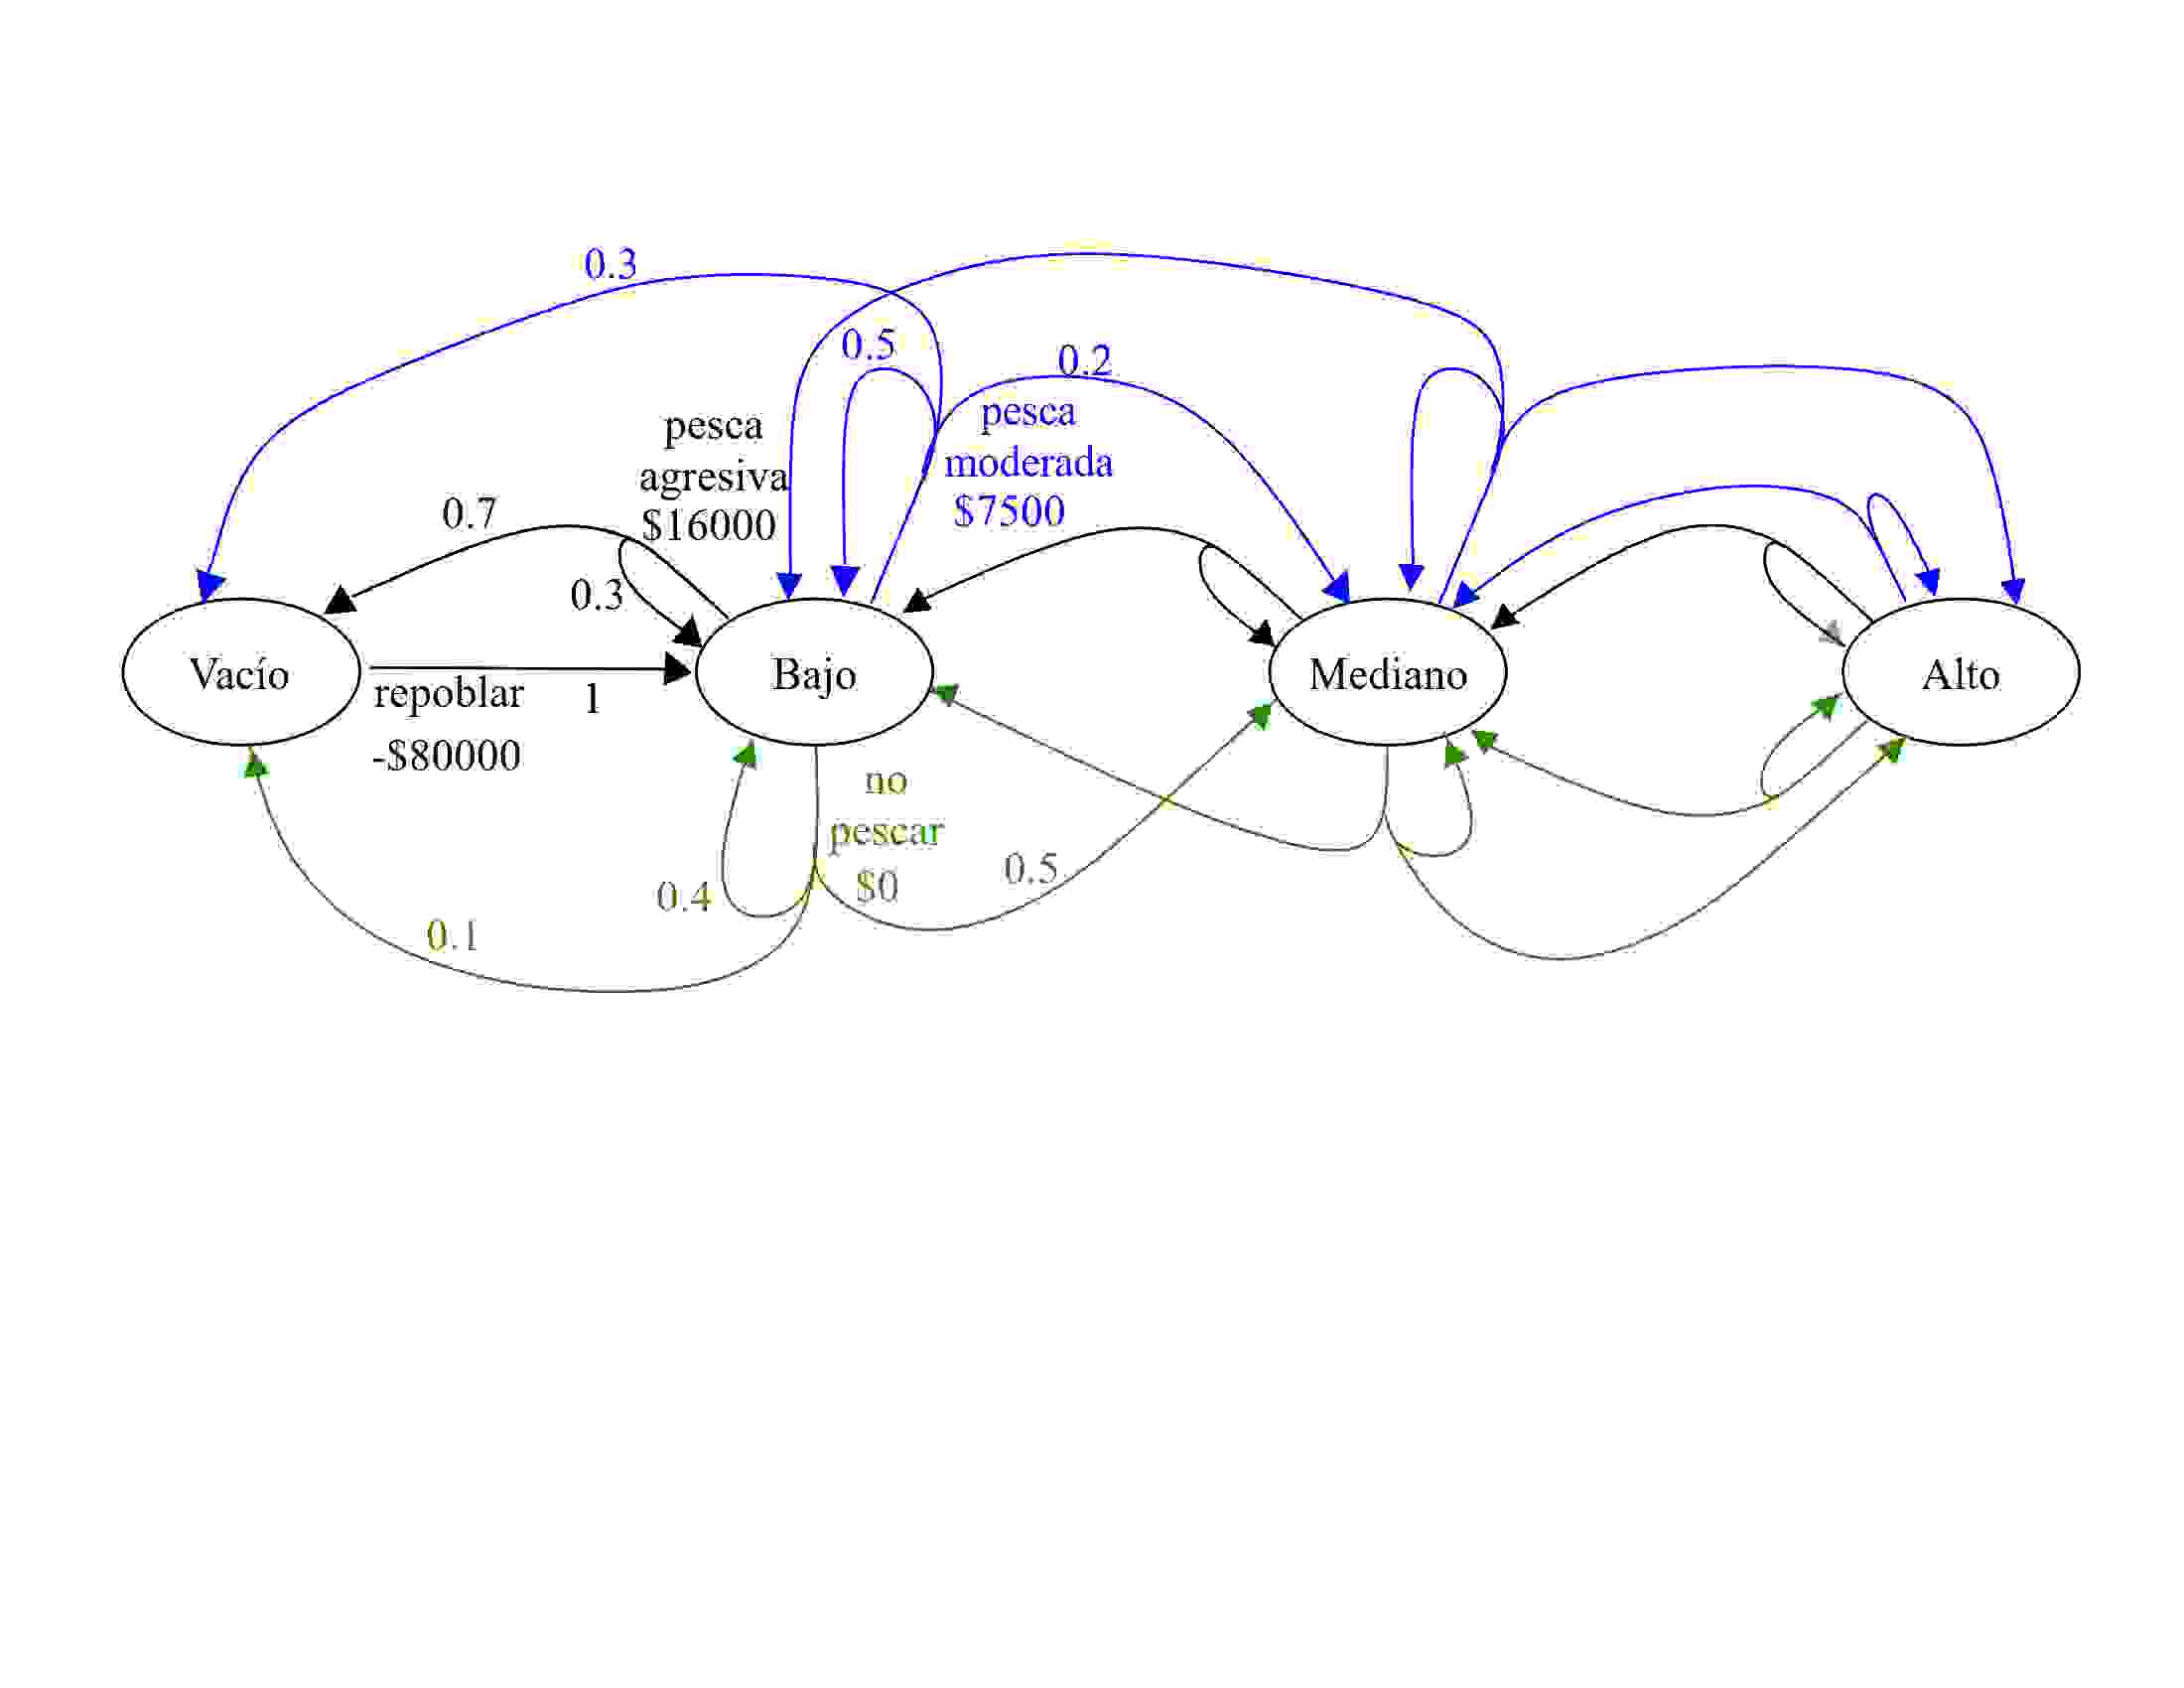
\includegraphics[width=1\textwidth]{../Images/SalmonFishing/SalmonFishing7.jpg}}
\end{center}
\vspace{-2cm}
\only<8>{Qué decisiones tomar? Vamos a resolver el problema con Python.}
\end{frame}

\begin{frame}{Pesca de Salmones: Resultados}
\begin{itemize}
\item Acá representamos la política óptima
\begin{itemize}
\item<2-> Acción óptima depende del estado y del tiempo
\end{itemize}
\item<3-> Cómo la elección del horizonte T impacta nuestras decisiones?
\end{itemize}
\begin{center}
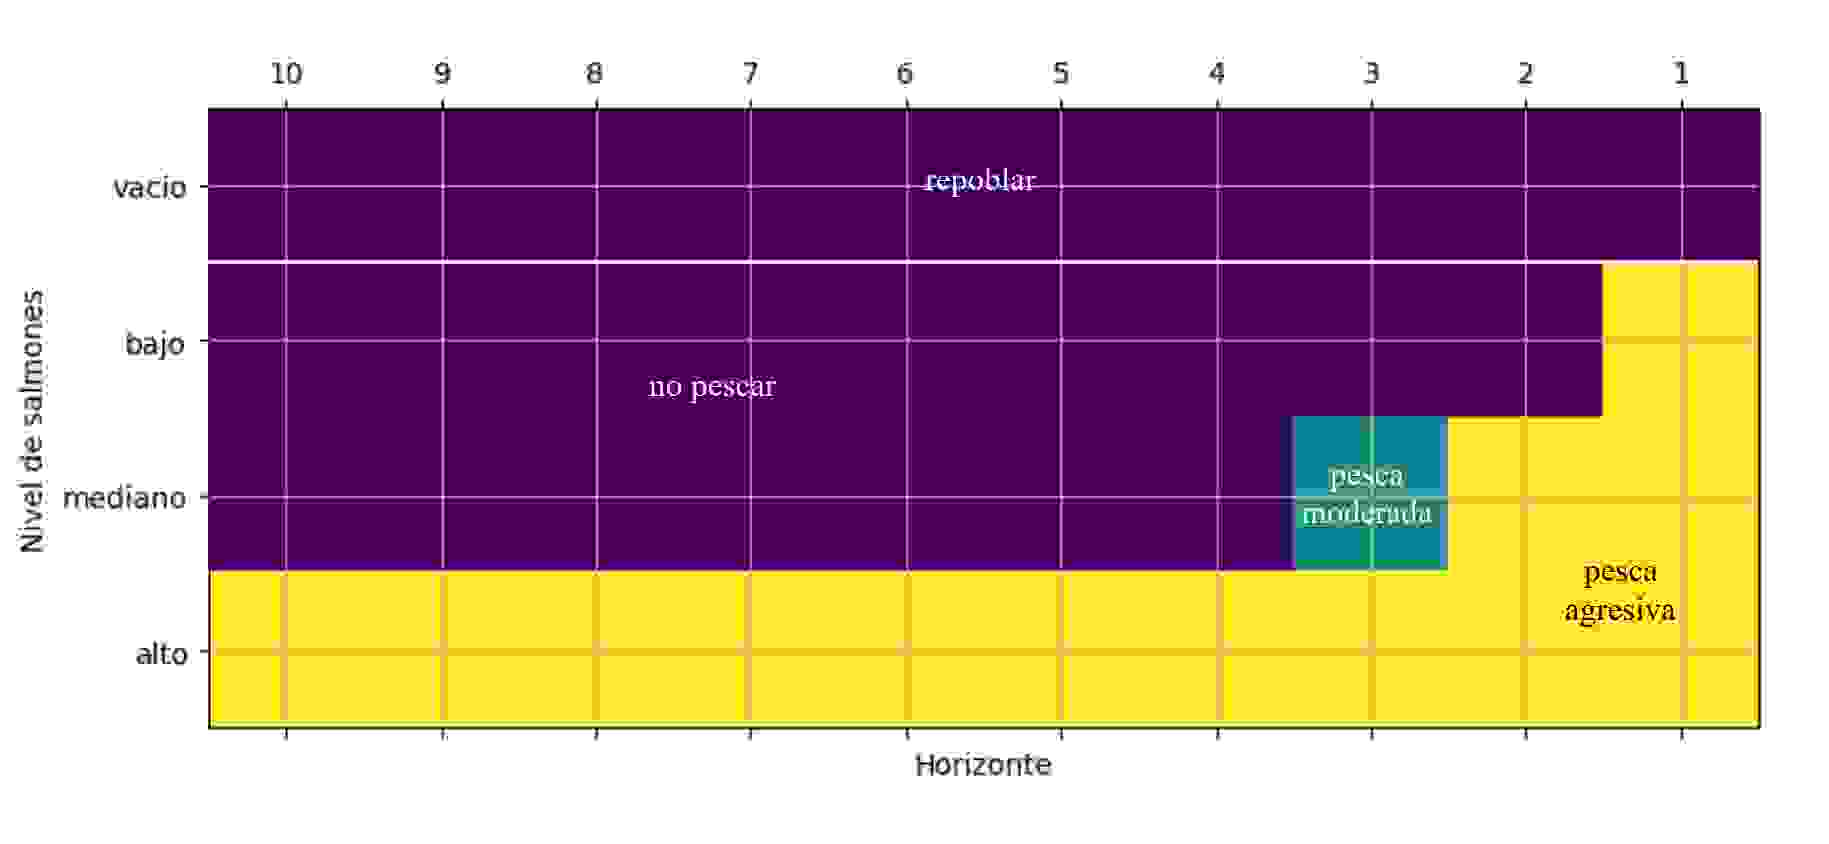
\includegraphics[width=1\textwidth]{../Images/SalmonFishing/SalmonFishingPolicy1.jpg}
\end{center}
\end{frame}

\begin{frame}{Pesca de Salmones: Opción de No Repoblar}
\begin{itemize}
\item<1->{Si en el estado vacío tenemos la opción de no repoblar, cómo eso cambia el análisis? Cuáles son las condiciones para repoblar o no?}
\end{itemize}
\begin{center}
\mode<beamer>{
\only<1>{
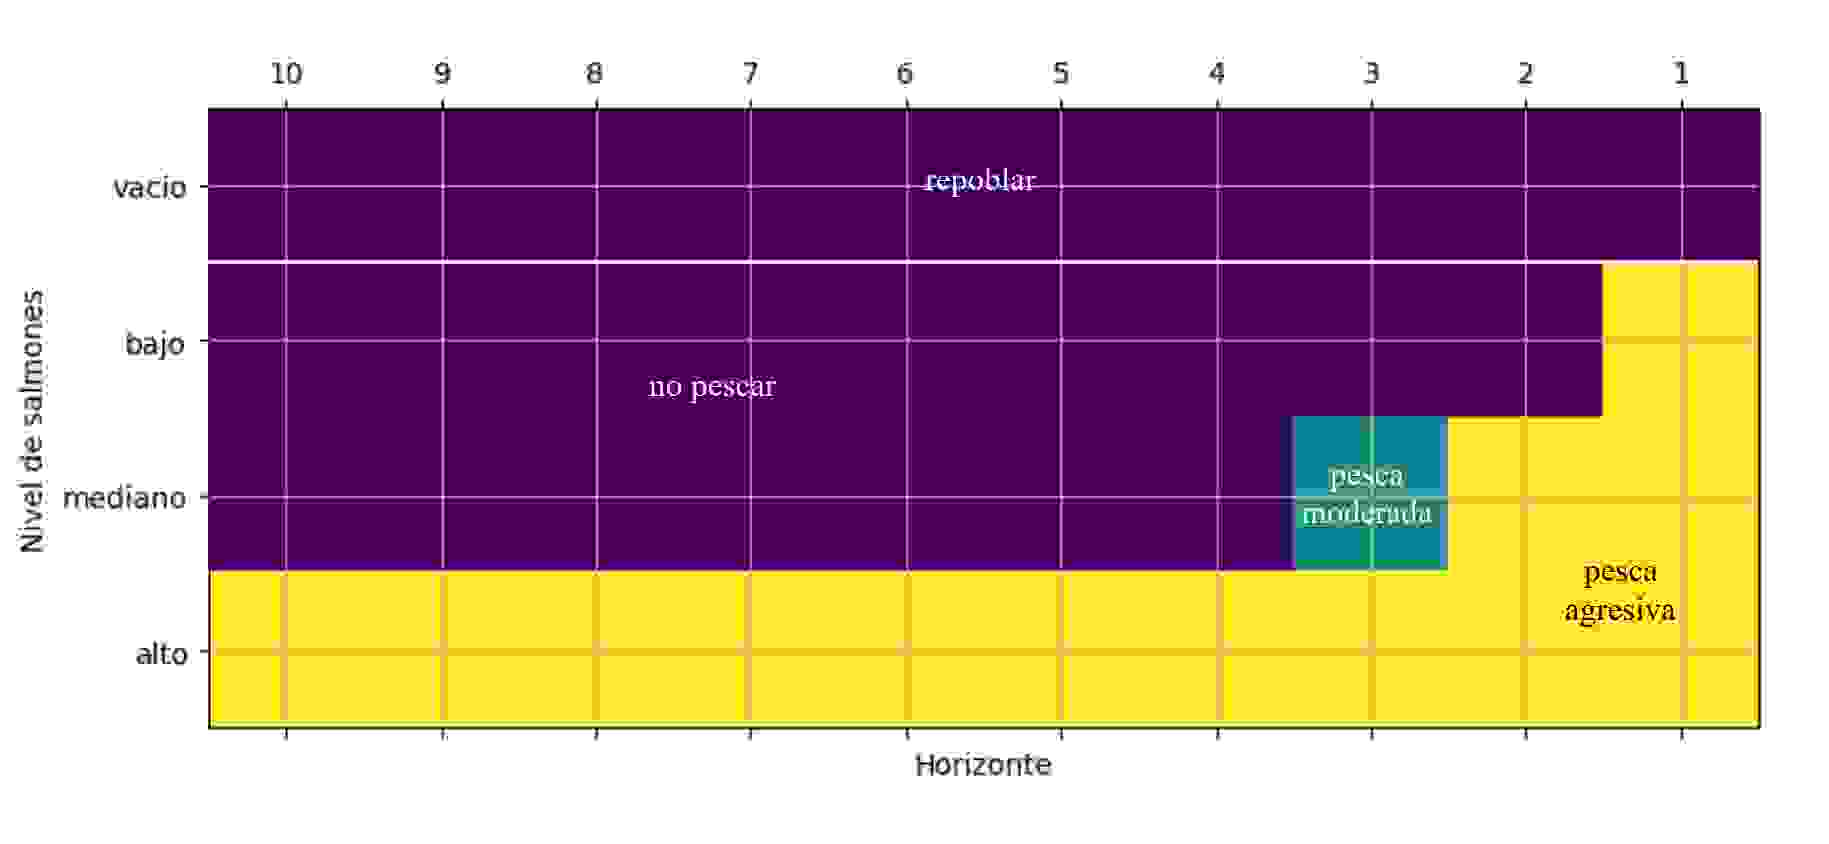
\includegraphics[width=1\textwidth]{../Images/SalmonFishing/SalmonFishingPolicy1.jpg}}}
\only<2>{
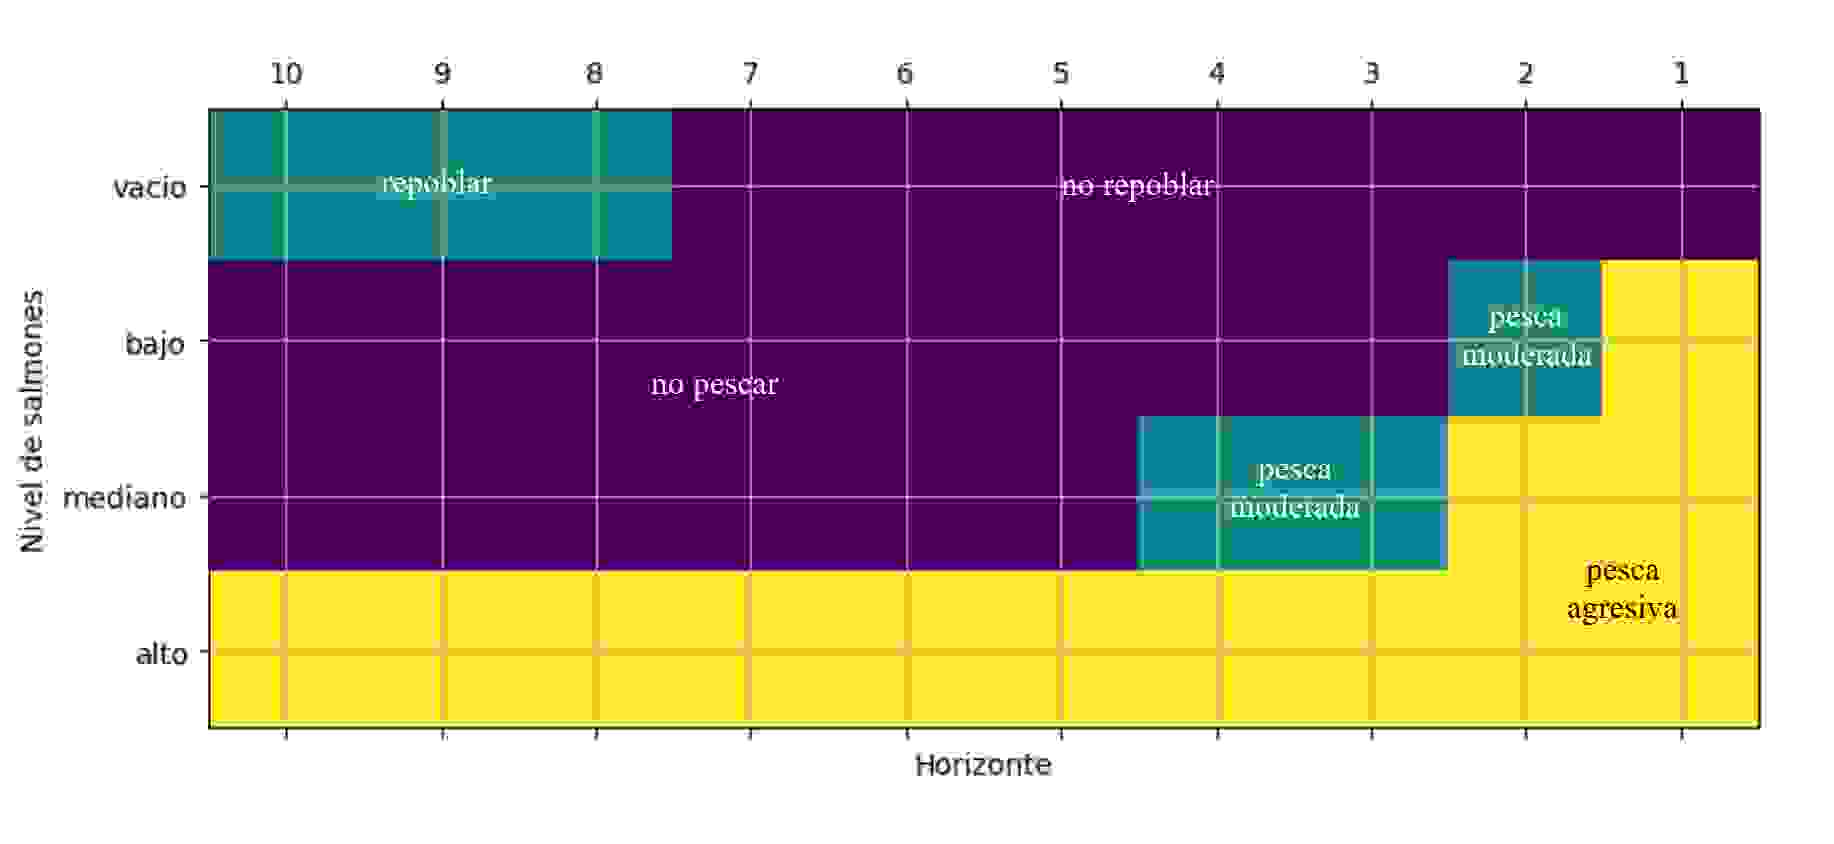
\includegraphics[width=1\textwidth]{../Images/SalmonFishing/SalmonFishingPolicy2.jpg}}
\end{center}
\end{frame}

\begin{frame}{Pesca de Salmones: Horizonte}
\begin{itemize}
\item Para obtener la política óptima, especificamos el horizonte $T$.
\begin{itemize}
\item<2-> La acción óptima depende de la distancia al horizonte.
\item<3-> Qué horizonte debemos elegir?
\item<4-> En algunas situaciones, la elección del horizonte es clara:
\begin{itemize}
\item Subastas
\item Campaña electoral
\item Logistica y operaciones con fecha de entrega
\item Precificació de pasajes aereos
\end{itemize}
\end{itemize}
\item<5-> Qué hacer si no hay una elección clara?
\item<6-> Podemos utilizar el horizonte infinito.
\end{itemize}
\end{frame}

\begin{frame}{MDPs con Horizonte Infinito}
\begin{itemize}
\item Vamos a considerar la ganancia esperada con $T=\infty$ y factor de descuento $\alpha$:
$$
\max_u {\rm E}\left[\sum_{t=0}^\infty \alpha^t r_u(x_t)\right]
$$
\begin{itemize}
\item<2-> factor de descuento $\alpha$ introduce preferencia entre ganancias próximas y ganancias futuras
\item<3-> también puede ser necesario para garantizar convergencia de la suma de ganancias
\item<4-> en muchas situaciones, se puede trabajar con $\alpha=1$ y considerar la ganancia promedio
$$
\max_u \lim_{T\rightarrow \infty} \frac{1}{T} {\rm E}\left[\sum_{t=0}^{T-1} r_u(x_t)\right]
$$
\end{itemize}
\item<5-> Cómo encontrar la política óptima?
\end{itemize}
\end{frame}

\begin{frame}{MDPs con Horizonte Infinito}
\begin{itemize}
\item Consideremos nuevamente la recursión utilizada con horizonte finito, con descuento.
\item<3-> Qué sucede cuando $T \mapsto \infty$?
\visible<4->{
$\lim_{T\mapsto\infty} V_t^* = V^*,~\forall t.$}
\only<6->{
\item Equación de Bellman:
$$V^*(x) =  \max\limits_{a \in A} \left\{r_a(x)+\alpha \sum_y P_a(x,y) V^*(y)\right\}$$}
\only<7->{
\item Si logramos resolver la ecuación de Bellman, podemos derivar nuevamente la política óptima a partir de la función valor:
$$u^*(x) =  \arg\max\limits_{a \in A} \left\{r_a(x)+\alpha \sum_y P_a(x,y) V^*(y)\right\}$$
\only<8->{\begin{itemize}
\item Notamos que $u^*$ no depende de $t$, la política óptima es estacionaria.
\end{itemize}}}
\end{itemize}
\mode<beamer>{
\only<2-5>{
\vfill
\begin{block}{Programación Dinámica con Horizonte T}
\begin{enumerate}
\item Hacemos $t = T$. Calculamos $V_T^*(x) = \max_a r_a(x).$
\item Hacemos $t = t-1$. Calculamos 
\only<1-3>{
$V^*_t(x) =  \max\limits_{a \in A} \left\{r_a(x)+\alpha \sum_y P_a(x,y) V_{t+1}^*(y)\right\}$.
}
\only<5>{
$\textcolor{red}{V^*}(x) =  \max\limits_{a \in A} \left\{r_a(x)+\alpha \sum_y P_a(x,y) \textcolor{red}{V^*}(y)\right\}$.
}
\item Si $t = 0$, fin. Si no, volvemos al paso 2.
\end{enumerate}
\end{block}}}
\end{frame}

\begin{frame}{Ecuación de Bellman - Iteración de Valor} 
\begin{itemize}
\item Hay varios algoritmos para resolver la ecuación de Bellman, nos enfocaremos en dos métodos que forman la base para los algoritmos de aprendizaje por refuerzo, iteración de valor e iteración de políticas.
\item<2-> Iteración de valor es básicamente el mismo algoritmo que el algoritmo de programación dinámica para horizonte finito:
\visible<3->{
\begin{block}{Iteración de Valor}
\begin{enumerate}
\item Hacemos $t = 0$. Inicializamos $V_0(x)$ con un valor arbitrario, por ejemplo $V_0(x) = 0~\forall x$.
\item Hacemos $t = t+1$. Calculamos 
$V_{t+1}(x) =  \max\limits_{a \in A} \left\{r_a(x)+\alpha \sum_y P_a(x,y) V_t(y)\right\}$.
\item Utilizando un criterio de convergencia para $V_t$, decidimos si parar o volver al paso 2.
\begin{itemize}
\item<4-> Por ejemplo, $\max_x |V_t(x)-V_{t-1}(x)|<\epsilon$ para algún $\epsilon>0$
\end{itemize}
\end{enumerate}
\end{block}}
\end{itemize}
\end{frame}

\begin{frame}{Ecuación de Bellman - Iteración de Política}
\begin{block}{Iteración de Política}
\begin{enumerate}
\item Hacemos $k = 0$. Empezamos con una política arbitraria $u_0$.

\item Evaluamos la función valor $V_{u_k}$ asociada con la política $u_k$. Para eso, debemos resolver:
$$
V_{u_k} = r_{u_k} + \alpha P_{u_k} V_{u_k}
$$
Calculamos una nueva política $u_{k+1}$, que será la \textbf{política codiciosa} con respeto a $V_{u_k}$:
$$
u_{k+1}(x) = \arg\max_{a \in A} \left\{r_a(x) + \alpha\sum_y P_a(x,y)V_{u_k}(y)\right\}
$$
\item Si $u_k=u_{k+1}$, paramos. Si no, hacemos $t = t+1$ y volvemos al paso 2.
\end{enumerate}
\end{block}
\end{frame}

\begin{frame}{Ecuación de Bellman - Iteración de Política - Intuición:}
\begin{itemize}
\item Tenemos
$u_{k+1}(x) = \arg\max_{a \in A} \left\{r_a(x) + \alpha\sum_y P_a(x,y)V_{u_k}(y)\right\}$
\only<2->{
entonces:
\only<2>{
$$
r_{u_{k+1}}+ \alpha P_{u_{k+1}}V_{u_k} \geq r_{u_k}+ \alpha P_{u_k}V_{u_k} = V_{u_k}
$$}
\visible<3->{
$$
\underbrace{r_{u_{k+1}}+ \alpha P_{u_{k+1}}V_{u_k}}_{{\rm valor~de~seguir}~(u_{k+1},u_k,u_k,\dots)} \geq \underbrace{r_{u_k}+ \alpha P_{u_k}V_{u_k}}_{{\rm valor~de~seguir}~(u_k,u_k,u_k,\dots)} = V_{u_k}
$$}}
\item<4->
La desigualdad es estricta por lo menos para un estado $x$, si $u_k$ no es una politica óptima
\only<5->{$\Rightarrow$ La política (no estacionaria) $(u_{k+1},u_k,u_k,\dots)$ es mejor que $(u_k,u_k,u_k,\dots)$.}
\item<6-> Siguiendo el mismo razonamiento, podemos demostrar que $(u_{k+1},u_{k+1},u_k,u_k,\dots)$ es mejor que $(u_{k+1},u_k,u_k,u_k,\dots)$.
\item<7-> Podemos seguir reemplazando $u_k$ con $u_{k+1}$ sucesivamente, obteniendo una secuencia de políticas que van mejorando.
\item<8-> Concluimos que $u_{k+1}$ es mejor que $u_k$.
\end{itemize}
\end{frame}

\begin{frame}{Políticas Rollout}
\begin{itemize}
\item Consideremos una única iteración de política:
\mode<beamer>{
\only<1-2>{
\begin{enumerate}
\item Evaluamos la función valor $V_{u_k}$ asociada con la política $u_k$
\item Calculamos una nueva política $u_{k+1}$, que será la \textbf{política codiciosa} con respeto a $V_{u_k}$:
$$
u_{k+1}(x) = \arg\max_{a \in A} \left\{r_a(x) + \alpha\sum_y P_a(x,y)V_{u_k}(y)\right\}
$$
\end{enumerate}}}
\only<3->{
\begin{enumerate}
\item Evaluamos la función valor $V_u$ asociada con una política $u$
\begin{itemize}
\item<4-> $u$ puede ser una heurística que ya se utiliza
\item<5-> $u$ y/o $V_u$ pueden ser el resultado de aprendizaje por refuerzo
\end{itemize}
\item<6-> Calculamos una nueva política $u_{{\rm rollout}}$, que será la \textbf{política codiciosa} con respeto a $V_{u}$:
$$
u_{{\rm rollout}}(x) = \arg\max_{a \in A} \left\{r_a(x) + \alpha\sum_y P_a(x,y)V_{u_k}(y)\right\}
$$
\end{enumerate}}
\mode<beamer>{
\item<2> Sabemos que $u_{k+1}$ es mejor que $u_k$.}
\item<7-> Sabemos que $u_{{\rm rollout}}$ es mejor que $u$.
\begin{itemize}
\item<8-> Opción práctica para mejorar heuristicas.
\item<9-> Utilizado en aplicaciones exitosas de aprendizaje por refuerzo, como TD-Gammon y AlphaGo
\end{itemize}
\end{itemize}
\end{frame}

\begin{frame}{Iteración de Valor vs Iteración de Política}
\begin{itemize}
\item Como hay un número finito de políticas, iteración de política siempre termina.

\item<2-> El número de políticas estacionarias es $|A|^{|S|}$. En el peor caso, la iteración de politica necesita un número de iteraciones que es exponencial en $|S|$, pero en la práctica, muchas veces termina en pocos pasos.

\item<3-> Un paso de iteración de política es más costoso que un paso de iteración de valor, porque debemos evaluar la política y seleccionar la nueva acción. 

\item<4-> Sin embargo, la iteración de política suele terminar en menos pasos, y la iteración de valor puede ser lenta, especialmente cuando el factor de descuento es alto.

\item<5-> Iteración de valor e iteración de política forman la base para muchos algoritmos de aprendizaje por refuerzo.
\end{itemize}
\end{frame}

\begin{frame}{Pesca de Salmones: Horizonte Infinito}
Resolución con horizonte infinito, distintos factores de descuento. Implementamos iteración de valor en Python...
\visible<2>{
\begin{center}
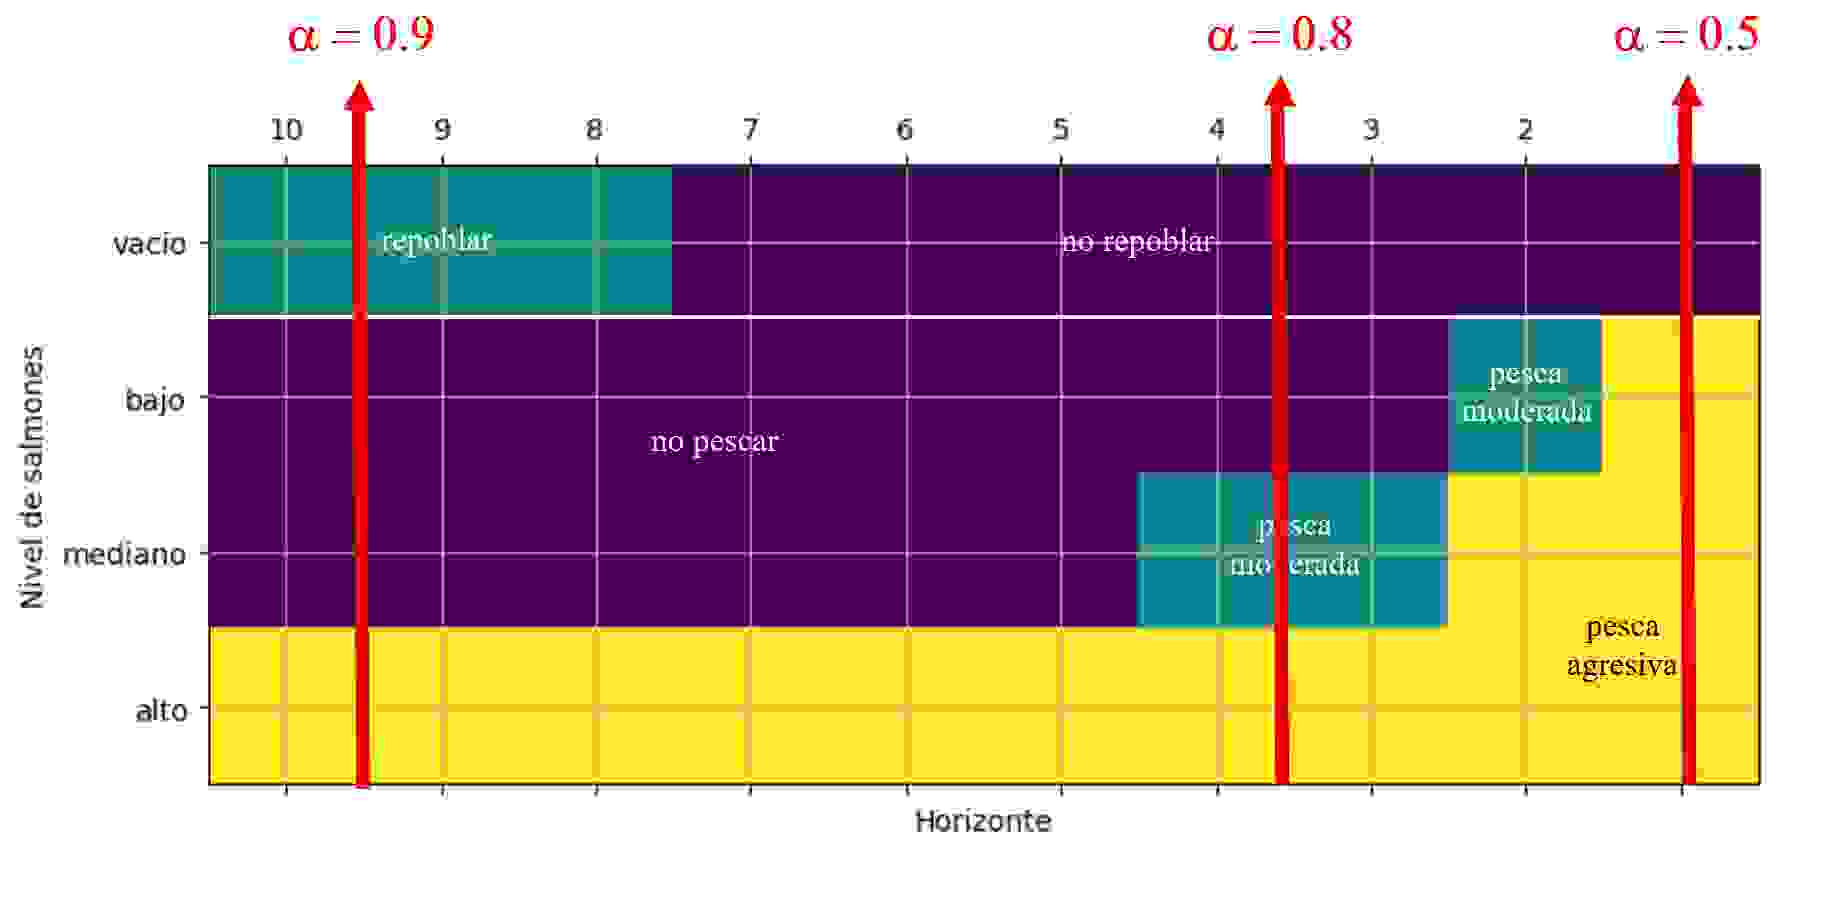
\includegraphics[width=1\textwidth]{../Images/SalmonFishing/SalmonFishingPolicy3.jpg}    
\end{center}
}
\end{frame}

\begin{frame}{Ejemplo: Optimización de Portafolio}
\begin{itemize}
\item Consideramos una situación donde hay dos posibilidades de inversión:
\begin{itemize}
\item una caja de ahorros con tasa de interés $r_f$;
\item un activo con precio $s_t$ que evoluciona en el tiempo según
$$s_{t+\Delta} = s_t e^{(r-\sigma^2/2)\Delta+\sigma \sqrt{\Delta} \epsilon_t}
$$
donde $\epsilon_t,~t = 0,1,...$ son variables aleatorias independientes y siguen la distribución normal estándar ($\epsilon_t \sim {\rm N}(0,1)$).
\begin{itemize}
\item<2-> Ese es el tradicional \textbf{modelo lognormal} para precios de activos.
\item<3-> $r$ es el rendimiento esperado del activo y $\sigma$ es su volatilidad.  
\end{itemize}
\end{itemize}
\item<4> Cómo debemos invertir para maximizar el valor del portafolio después de un periodo $T$?
\end{itemize}
\end{frame}

\begin{frame}{Modelo Lognormal Para Precios - Tiempo Discreto}
\begin{itemize}
\item El modelo lognormal para precios es válido para cualquier $t$ y $\Delta$: $s_{t+\Delta} = s_t. e^{(r-\sigma^2/2)\Delta+\sigma\sqrt{\Delta}\epsilon_t}$
donde $\epsilon_t,~t = 0,1,...$ son variables aleatorias independientes y siguen la distribución normal estándar ($\epsilon_t \sim {\rm N}(0,1)$).
\item<2-> Vamos a considerar el modelo a tiempo discreto, con $t = 0, \Delta, 2\Delta,\dots$ para un valor fijo de $\Delta$. Consideremos que tomamos decisiones solamente en esos momentos discretos.
\item<3-> Noten que:
$$
\begin{array}{ccl}
s_{t+\Delta} & = & s_t e^{(r-\sigma^2/2)\Delta+\sigma\sqrt{\Delta}\epsilon_t} \\
& = & s_t e^{(r\Delta -(\sigma\sqrt{\Delta})^2/2+\sigma\sqrt{\Delta}\epsilon_t} \\
& = & s_t e^{\tilde{r}-\tilde\sigma^2/2+\tilde\sigma \epsilon_t}
\end{array}
$$
donde $\tilde r  = r \Delta$ y $\tilde \sigma = \sigma \sqrt{\Delta}$.
\item<4-> Entonces podemos considerar el modelo a tiempo discreto:
$$
\tilde s_{n+1} = \tilde s_n e^{\tilde r-\tilde \sigma^2/2+\sigma\epsilon_n}
$$
donde $\epsilon_n \sim {\rm N}(0,1)$ y $\tilde s_n = s_{n\Delta}$.
\end{itemize}
\end{frame}

\begin{frame}{Modelo Lognormal Para Precios - Tiempo Discreto}
\begin{itemize}
\item Modelo a tiempo discreto:
$$
s_{n+1} = s_n e^{r- \sigma^2/2+\sigma\epsilon_n}
$$
donde $\epsilon_n \sim {\rm N}(0,1)$ y $\tilde s_n = s_{n\Delta}$. (Sacamos los tildes para simplificar la notación.)
\item<2-> Ejemplo: Si un activo tiene rendimiendo esperado anual de 10\% y volatilidad de 40\%, y consideramos rebalancear el portafolio una vez por mes, cómo modelamos su precio?
\begin{itemize}
\item<3-> Cada periodo corresponde a $\Delta = 1/12$ (un mes).
\item<4-> El rendimiento mensual tiene valor esperado y volatilidad de
$$r = 0.1/12 \approx 0.0083,~\sigma = 0.4\sqrt{1/12} \approx 0.1155$$ 
\item<5-> La evolución del precio del activo mes a mes es dada por 
$$
s_{t+1} = s_te^{0.0083-0.1155^2/2+0.1155\epsilon_t} = s_te^{0.0016+0.1155\epsilon_t}.
$$
\end{itemize}
\end{itemize}
\end{frame}

\begin{frame}{Optimización de Portafolio: Modelo MDP $(S,A,P,r)$}
\begin{itemize}
\item Estado: \visible<2->{valor $W_t$ del portafolio}
\item<3-> Acción: \visible<4->{fracción $\beta_t$ del portafolio invertida en la acción} 
\item<5-> Transición: \visible<6->{$W_{t+1}=W_t\left(\beta_t e^{r-\sigma^2/2+\sigma \epsilon_t}+(1-\beta_t)e^{r_f}\right)$}           
\item<7-> Recompensa/Criterio de optimalidad?
\begin{itemize}
\item<8-> Empezamos maximizando el valor del portafolio al final de $T$ periodos:
$$
\max_u {\rm E}\left[W_T\right]
$$
\item<9-> $r_T(w) = w$ $r_t(w) = 0,~\forall t < T$.
\item<10-> Maximizar el valor final esperado del portafolio es solo una opción, hay muchas formulaciones posibles.
\end{itemize}
\end{itemize}
\end{frame}
\begin{frame}{Optimización de Portafolio: Función Valor y Recursión}
\begin{itemize}
\item La función valor es $V_t^*(w) = {\rm E}\left[W_T| W_t = w\right]$
\begin{itemize}
\item valor esperado del portafolio en el periodo $T$ dado el valor actual $w$. 
\end{itemize}
\item<2-> La ecuación de Bellman es:
$$
\begin{array}{ccl}
V_T^*(w) & = & w \only<3->{\\
V_t^*(w) & = &\max\limits_{\beta \in [0,1]}{\rm E}\left[V_{t+1}^*(W_{t+1})|W_t = w\right]}
\only<4->{\\
&= & \max\limits_{\beta \in [0,1]}{\rm E}\left[V_{t+1}^*\left(w\left[\beta e^{r-\sigma^2/2+\sigma \epsilon_t}+(1-\beta)e^{r_f}\right]\right)\right]}
\end{array}
$$
\only<4->{donde utilizamos la transición $W_{t+1}=W_t\left(\beta_t e^{r-\sigma^2/2+\sigma \epsilon_t}+(1-\beta_t)e^{r_f}\right)$.}
\item<5-> En este ejemplo, el espacio de estados es continuo y la transición está representada por una función, en vez de la matriz de transición $P$.
\begin{itemize}
\item<6-> Debemos evaluar ${\rm E}[V_{t+1}^*(w_{t+1})]$, que en este caso no se expresa como $\sum_y P_\beta(w,w') V_{t+1}^*(w')$.
\end{itemize}
\end{itemize}
\end{frame}

\begin{frame}{Optimización de Portafolio: Solución}
Vamos a utilizar recursión, ya que el horizonte es finito.
\begin{itemize}
\item<2->En el periodo final, recibimos $V^*_T(w) = w$.
\item<3-> En $t = T-1$, debemos optimizar:
$$
\begin{array}{ccl}
V_{T-1}^*(w) & = & \max\limits_{\beta \in [0,1]} {\rm E}\left[V_T^*\left(w\left[\beta e^{r-\sigma^2/2+\sigma \epsilon_{T-1}}+(1-\beta)e^{r_f}\right]\right)\right] \\
\visible<4->{& = &\max\limits_{\beta \in [0,1]} {\rm E}\left[w\left(\beta e^{r-\sigma^2/2+\sigma \epsilon_{T-1}}+(1-\beta)e^{r_f}\right)\right]\\}
\visible<5->{& = & w \max\limits_{\beta \in [0,1]}{\rm E}\left[\left(\beta e^{r-\sigma^2/2+\sigma \epsilon_{T-1}}+(1-\beta)e^{r_f}\right)\right] \\}
\visible<6,8->{& = & w \max\limits_{\beta \in [0,1]}\left\{\beta e^{r-\sigma^2/2} {\rm E}\left[e^{\sigma \epsilon_{T-1}}\right]+(1-\beta)e^{r_f}\right\} \\}
\only<7>{& = & w \max\limits_{\beta \in [0,1]}\{\beta e^{r-\sigma^2/2} \underbrace{{\rm E}\left[e^{\sigma \epsilon_{T-1}}\right]}_{e^{\sigma^2/2}}+(1-\beta)e^{r_f}\} \\}
\visible<8->{& = & w\max\limits_{\beta \in [0,1]} \left\{\beta e^r + (1-\beta)e^{r_f}\right\}}
\end{array}
$$
\item<9-> Tenemos:
\begin{itemize}
    \item $\beta_{T-1}^*(w) = 1$ si $r>r_f$ y 0 si $r<r_f$, independiente de $w$;
    \item $V_{T-1}^*(w) = w \max(e^r, e^{r_f}) = w C$
    \begin{itemize}
    \item<10-> \textcolor{red}{$V_{T-1}^*$ es lineal en $w$.}
    \end{itemize}
\end{itemize}
\end{itemize}
\end{frame}

\begin{frame}{Optimización de Portafolio: Solución}
Vamos a utilizar recursión, ya que el horizonte es finito.
\begin{itemize}
\item En el periodo final, recibimos $V^*_T(w) = w$.
\item En \textcolor{red}{$t = T-2$}, debemos optimizar:
$$
\begin{array}{ccl}
V_{\textcolor{red}{T-2}}^*(w) & = & \max\limits_{\beta \in [0,1]} {\rm E}\left[V_{\textcolor{red}{T-1}}^*\left(w\left[\beta e^{r-\sigma^2/2+\sigma \epsilon_{\textcolor{red}{T-2}}}+(1-\beta)e^{r_f}\right]\right)\right]\\
& = &\max\limits_{\beta \in [0,1]} {\rm E}\left[\textcolor{red}{C} w\left(\beta e^{r-\sigma^2/2+\sigma \epsilon_{\textcolor{red}{T-2}}}+(1-\beta)e^{r_f}\right)\right]\\
& = & \textcolor{red}{C} w \max\limits_{\beta \in [0,1]}{\rm E}\left[\left(\beta e^{r-\sigma^2/2+\sigma \epsilon_{\textcolor{red}{T-2}}}+(1-\beta)e^{r_f}\right)\right] \\& = & \textcolor{red}{C}w \max\limits_{\beta \in [0,1]}\left\{\beta e^{r-\sigma^2/2} {\rm E}\left[e^{\sigma \epsilon_{\textcolor{red}{T-2}}}\right]+(1-\beta)e^{r_f}\right\} \\& = & \textcolor{red}{C}w\max\limits_{\beta \in [0,1]} \left\{\beta e^r + (1-\beta)e^{r_f}\right\} 
\end{array}
$$
\item Tenemos:
\begin{itemize}
    \item $\beta_{\textcolor{red}{T-2}}^*(w) = 1$ if $r>r_f$ y 0 si $r<r_f$, independiente de $w$;;
    \item $V_{\textcolor{red}{T-2}}^*(w) = \textcolor{red}{C} w \max(e^r, e^{r_f}) = C^{\textcolor{red}{2}}w$
    \begin{itemize}
    \item \textcolor{red}{$V_{T-2}^*$ es lineal en $w$.}
    \item<2-> Podemos seguir el mismo argumento con $t = T-3,...,$.
    \end{itemize}
\end{itemize}
\end{itemize}
\end{frame}

\begin{frame}{Optimización de Portafolio: Solución}
\begin{itemize}
\item Del desarrollo anterior, concluimos que la función valor tiene la forma:
$$
V_t^*(w) = w \max(e^r, e^{r_f})^{T-t}.
$$
\item<4-> Entonces, la política óptima no depende del tiempo ni del valor del portafolio: 
$$
\beta_{t}^*(w) = \beta* = \begin{cases}
1 & {\rm si~} r>r_f \\
0 & {\rm si~} r<r_f \\
{\rm cualquier~valor} &{\rm si~}r=r_f
\end{cases}
$$
\end{itemize}
\end{frame}

\begin{frame}{Optimización de Portafolio: Observaciones}
\begin{itemize}
\item En ese ejemplo, la solución es simple e intuitiva, reduciéndose a maximizar el rendimiento esperado en cada período. 
\begin{itemize}
\item<2-> Eso se debe a que el rendimiento del activo es independiente y distribuido igualmente a cada periodo.
\end{itemize}
\item<3-> La metodología puede ser aplicada en condiciones más complejas, por ejemplo:
\begin{itemize} 
\item<4-> la tasa de interés, el rendimiendo de la acción y su volatilidadd pueden ser fluctuantes;
\item<5-> pueden haber costos para realizar transacciones.
\end{itemize}
\item<6-> En este caso tanto la variable de estado como la acción son contínuas.
\begin{itemize}
\item<7-> Si una solución analítica no existe, necesitamos realizar aproximaciones, por ejemplo discretizando el espacio de estados y/o el espacio de acciones.
\end{itemize}
\end{itemize}
\end{frame}

\begin{frame}{Repensando La Función Recompensa}
\begin{itemize}
\item Maximizando el valor esperado final ${\rm E}\left[W_T\right]$, la optimización en cada período $t$ se reduce a
$$
\max\limits_{\beta \in [0,1]} \left\{\beta e^r + (1-\beta)e^{r_f}\right\} 
$$
\item<2-> Comparación simple entre el rendimiento esperado $r$ del activo y la tasa de interés $r_f$.
\item<3-> Independiente de la volatilidad $\sigma$ del instrumento de riesgo.
\item<4-> Pero: $R_{\rm riesgo} = e^{r-\sigma^2/2+\sigma \epsilon}$, donde $\epsilon \sim {\rm N}(0,1)$, y $R_{\rm ahorro} = e^{r_f}$
\item<5-> Vamos a comparar $R_{\rm riesgo}$ y $R_{\rm ahorro}$ con distintos valores de $\sigma$...
\end{itemize}
\end{frame}

\begin{frame}{Repensando La Función Recompensa}
\begin{itemize}
\item<1-> $R_{\rm riesgo} = e^{r-\sigma^2/2+\sigma \epsilon}$, , donde $\epsilon \sim {\rm N}(0,1)$, y $R_{\rm ahorro} = e^{r_f}$
\item<2-> Generamos la distribución de $R_{\rm riesgo}$ con Python...
\visible<3->{
\begin{center}
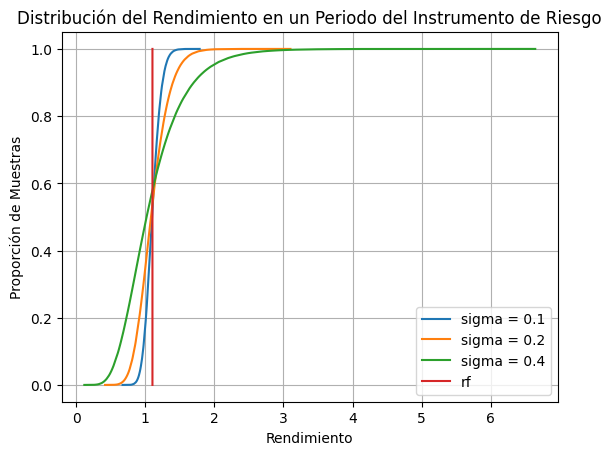
\includegraphics[width=0.8\textwidth]{../Images/Portfolios/StockReturns.png}
\end{center}}
\item<4-> Somos indiferentes a esas cuatros opciones?
\end{itemize}
\end{frame}

\begin{frame}{Aversión al Riesgo}
\begin{itemize}
\item Consideremos una situación donde podés elegir recibir un monto fijo o un monto establecido por el resultado de tirar una moneda. 
\item Si el monto fijo es \$500 y el monto dado por la moneda es \$0 o \$1000, qué elegís?
\item<2-> Si el monto fijo es US\$500,000 y el monto dado por la moneda es US\$0 o US\$1,000,000, qué elegís?
\end{itemize}
\end{frame}

\begin{frame}{Función de Utilidad}
\begin{itemize}
\item Podemos capturar nuestras preferencias respecto al riesgo eligiendo la función de recompensa con el concepto de \textbf{función de utilidad}. 
\item<2->La función de utilidad captura el valor de distintas opciones. Por ejemplo, en el caso del juego con la moneda, podemos elegir $\nu(w) = \log(0.001w+1)$.
\begin{center}
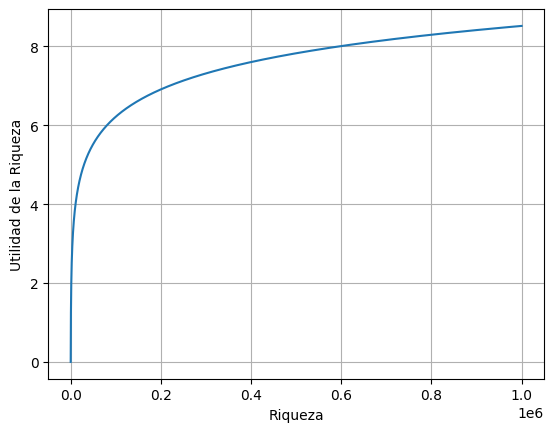
\includegraphics[width=0.4\textwidth]{../Images/Portfolios/UtilityFunction.png}
\end{center}
\item<3-> Por qué cóncava?
\item<4->Entonces:
$$
\begin{array}{l}
u(0.5) \approx 0.5(u(0)+u(1))\approx 0.0005\\
u(500000) = 6.2166 > 0.5(u(0)+u(1000000)) = 3.4544
\end{array}
$$
\end{itemize}
\end{frame}

\begin{frame}{Función de Utilidad}
\begin{itemize}
\item Vamos a aplicar la función de utilidad $u(w) = w^\gamma/\gamma$, donde $0<\gamma\leq 1$.
\item<2-> Funciones con {\bf aversión relativa constante al riesgo}
\begin{itemize}
\item<3-> $u(aw) = a^\gamma u(w)$
\item<4-> preferencia relativa $u(aw)/u(w) = a^\gamma$ no depende de $w$. 
\end{itemize}
\item<5-> Casos límite:
\begin{itemize}
\item<6-> Con $\gamma = 1$, $u(w) = w$, utilidad neutral al riesgo
\item<7-> $\lim_{\gamma\rightarrow 0} u(w) = \log(w)$
\end{itemize}
\end{itemize}
\only<8->{
\begin{center}
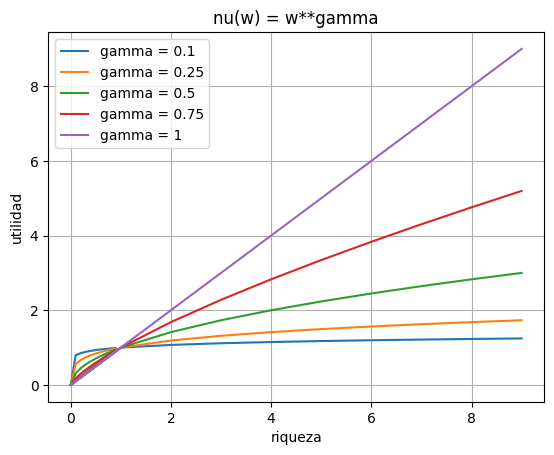
\includegraphics[width=0.5\textwidth]{../Images/Portfolios/UtilityFunction2.png}    
\end{center}}
\end{frame}

\begin{frame}{Optimización de Portafolio con Función de Utilidad}
\begin{itemize}
\item Nuestro criterio se vuelve:
$\max_u {\rm E}\left[\nu(W_T)\right] = \max_u {\rm E}\left[W_T^\gamma\right]$.
\item<2-> Podemos seguir los mismos pasos que utilizamos en la maximización del valor esperado ${\rm E}[W_T]$ para determinar que:
$$
V_t^*(w) = w^\gamma \left\{\max\limits_{\beta \in [0,1]}{\rm E}_{\epsilon\sim{\rm N}(0,1)}\left[\left(\beta e^{r-\sigma^2/2+\sigma \epsilon}+(1-\beta)e^{r_f}\right)^\gamma\right]\right\}^{T-t}
$$
\item<4-> Entonces, la política óptima es constante en el tiempo e independiente de la riqueza: 
$$
\beta_{\gamma,t}^*(w) = \beta_\gamma^* = \arg\max\limits_{\beta \in [0,1]}{\rm E}_{\epsilon\sim{\rm N}(0,1)}\left[\left(\beta e^{r-\sigma^2/2+\sigma \epsilon}+(1-\beta)e^{r_f}\right)^\gamma\right]
$$
\item<5-> Calculamos $\beta_\gamma^*$ con Python...
\end{itemize}
\end{frame}

\begin{frame}{Optimización de Portafolio con Función de Utilidad}
\begin{itemize}
\item $r_f = 0.04$, $r = 0.1$
\begin{center}
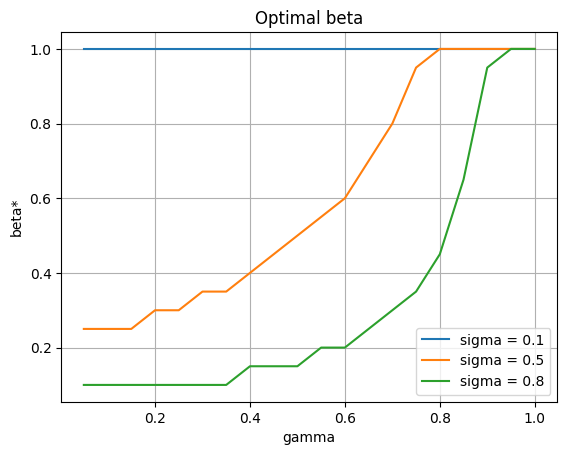
\includegraphics[width=0.9\textwidth]{../Images/Portfolios/BetaStar.png}
\end{center}
\end{itemize}
\end{frame}

\begin{frame}{Optimización de Portafolio con Consumo}
\begin{itemize}
\item Ahora asumimos que podemos gastar una parte de la riqueza a cada periodo. 
\item<2-> Modelo MDP?
\begin{itemize}
\item<3-> Estado = valor $W_t$ del portafolio
\item<4-> Acción: $0\leq \beta_t \leq 1$, $0\leq \delta_t \leq 1$  
\begin{itemize}
\item<5-> En cada periodo t, consumimos $\delta_t W_t$ e invertimos una fracción $\beta_t$ del restante en el activo y $1-\beta_t$ en la caja de ahorros. 
\end{itemize}
\item<6-> Transición: $W_{t+1} = (1-\delta_t) W_t \left[\beta_t e^{r-\sigma^2/2+\sigma \epsilon_t}+(1-\beta_t)e^{r_f}\right]$
\item<7-> Recompensa: $\nu(\delta_t W_t)$
\item<8-> Criterio de optimalidad: $\max_u \left[\sum_{t=0}^T \alpha^t \nu(\delta_t W_t)\right]$.
\end{itemize}
\item<9-> Ecuación del Bellman:
{\small
$$
\hspace{-1.5cm}V^*(w) = \max\limits_{\beta,\delta} \left\{ \nu(\delta w) + \alpha {\rm E}_{\epsilon \sim {\rm N}(0,1)}\left[V^*\left((1-\delta) w \left[\beta e^{r-\sigma^2/2+\sigma \epsilon}+(1-\beta)e^{r_f}\right]\right)\right]\right\}
$$}
\end{itemize}
\end{frame}

\end{document}
